\documentclass[pdflatex,sn-basic]{sn-jnl}

\usepackage{mathptmx}
\usepackage{graphicx}
\usepackage{multirow}
\usepackage{manyfoot}
\usepackage{textcomp}
\usepackage{amsmath,amssymb,amsfonts}
\usepackage{booktabs}
\usepackage{array}
\usepackage{xcolor}
\usepackage{algorithm}
\usepackage{algpseudocode}
\renewcommand{\algorithmicrequire}{\textbf{Input:}}
\renewcommand{\algorithmicensure}{\textbf{Output:}}
\graphicspath{{figures/}}

\raggedbottom

\begin{document}

\title[Stagnation-triggered interventions for wrapper feature selection]{Stagnation-Triggered Interventions for Wrapper Feature Selection: RL-DOHO and a Controlled Test of Learned Operator Selection}

\author*[1]{\fnm{Preetha} \sur{Evangeline D}}\email{preethaevangeline.d@vit.ac.in}
\author[1]{\fnm{Prasenjit} \sur{Choudhury}}\email{prasenjit.choudhury2023@vitstudent.ac.in}
\author[1]{\fnm{Shreyansh} \sur{Dabgar}}\email{shreyansh.dabgar2023@vitstudent.ac.in}
\author[1]{\fnm{Aditya} \sur{Jha}}\email{aditya.jha2023@vitstudent.ac.in}

\affil*[1]{\orgdiv{School of Computer Science and Engineering}, \orgname{Vellore Institute of Technology}, \orgaddress{\city{Chennai}, \postcode{600127}, \state{Tamil Nadu}, \country{India}}}

\abstract{In wrapper feature selection, population-based search tends to stall long before its budget is used. We study a remedy: a stagnation-triggered intervention layer that, after a few stalled iterations, applies one of a small set of moves: a tabu-guarded bit-flip search around the best subset, a partial restart or a second optimizer's iteration. We instantiate it as RL-DOHO, a hybrid of the Dandelion Optimizer (DO) and Hippopotamus Optimization (HO) in which a UCB1 bandit chooses the move. On eleven clinical, gene-expression and tabular datasets, with equal budgets, ten seeds and pre-specified hypotheses, RL-DOHO reached lower fitness than the published DO in 103 of 110 paired runs (4 losses), and stayed ahead when DO was given larger steps or a sigmoid encoding, at the largest step only on gene data. It was level with HO (58 against 49), while a genetic algorithm (GA) did better more often (85 against 22). Added to HO, the same layer improved it in 71 runs against 29 ($p<0.001$); added to the GA, it changed nothing. Learned move selection added nothing: UCB1, tabular Q-learning and random choice were level, and neither a warm start nor a reward aimed at the best subset changed that, even though the bandit then learned to favour the most successful moves. Early intervention beat waiting; on low-dimensional data the bit-flip search alone was strongest. Tabular results replicated with a second classifier; no test-accuracy difference survived correction. The contribution is the intervention layer and a controlled negative result on learned operator selection.}

\keywords{Wrapper feature selection, Memetic algorithm, Adaptive operator selection, Multi-armed bandit, Dandelion optimizer, Hippopotamus optimization}

\maketitle

\section{Introduction}

Wrapper feature selection scores each candidate subset by training the classifier that will later use it. This keeps the selection honest to the model, but it turns the task into a search over $2^D-1$ subsets for $D$ features \citep{kohavi1997,xue2016}. Metaheuristics such as genetic algorithms, PSO or grey wolf optimization are popular for this search because they need fitness values and nothing else. In our own runs, however, they showed a common pattern: the population converged on one subset fairly early, and much of the remaining budget went on candidates that reproduced that subset.

A natural fix is to watch for that moment and do something different when it comes. What to do at that point is less clear. Several recent methods leave the decision to a learned controller, typically a multi-armed bandit or a Q-learning agent \citep{fialho2010,karafotias2015,hu2023rlgwo,hashjin2025q2ho}. Such controllers are not always compared with simply choosing the move at random, so it is often unclear whether the learning or the intervention does the work.

We study both questions on one concrete method. RL-DOHO runs the published Dandelion Optimizer (DO) \citep{zhao2022do} while the best subset improves and, after $\kappa$ stalled iterations, lets a UCB1 bandit \citep{auer2002} choose among a bit-flip search around the best subset, a partial restart, a DO iteration and a Hippopotamus Optimization (HO) \citep{amiri2024ho} iteration. A bandit is the stateless case of reinforcement learning \citep{sutton2018}, hence the name. We evaluate it on eleven datasets: a 12,085-patient rheumatic and autoimmune disease dataset \citep{mahdi2025data}, on which most methods reach similar accuracy, five gene-expression datasets with thousands of features, and five medical tabular datasets.

Our contributions are as follows:
\begin{itemize}
\item A stagnation-triggered intervention layer for wrapper search, and its instantiation as RL-DOHO with the published DO and HO update rules, tabu memory and a sparse start for high-dimensional data.
\item An equal-budget benchmark against ten other methods on eleven datasets. Hypotheses were fixed ahead of the runs that test them, and negative outcomes are reported alongside the positive ones.
\item A component analysis: the same layer on HO and on a genetic algorithm (GA), the trigger $\kappa$, each move on its own, a second classifier and repeated clinical splits.
\item A controlled test of learned operator selection. UCB1, tabular Q-learning, a warm-started UCB1 and a UCB1 with a reward aimed at the best subset were compared with random choice, and none helped. The diagnostics explain why. With a suitable reward the bandit learned which moves were better, but even the best move improved the best subset in at most 28\% of its uses, so the learned preference had little to work with.
\end{itemize}

In brief, the layer is what helps: RL-DOHO is better than DO, also when DO is given larger steps or a sigmoid encoding, and level with HO, the layer also improves HO, and a random choice of move works as well as a learned one. A GA reached lower fitness more often, and no method was significantly better on held-out data. Section~\ref{sec:related} reviews related work, Section~\ref{sec:method} describes the method, Section~\ref{sec:setup} the protocol, Section~\ref{sec:results} the results and Section~\ref{sec:discussion} their interpretation and limits.


\section{Related Work}\label{sec:related}

\subsection{Wrapper feature selection with metaheuristics}
Surveys of evolutionary feature selection \citep{xue2016} show that genetic algorithms, particle swarm optimization (PSO) and grey wolf optimization (GWO) are among the most used wrapper searches. Binary versions of PSO \citep{kennedy1997} and GWO \citep{mirjalili2014gwo,emary2016bgwo} map continuous positions to bits through transfer functions. Hybrids that add local search to a population method are also common; for example, the whale optimization algorithm has been combined with simulated annealing \citep{mafarja2017}. The no-free-lunch theorems \citep{wolpert1997} say that, averaged over all problems, no search method beats another. This is often given as a reason to build hybrids; we read it equally as a reason to compare any hybrid with plain baselines. Reviews of feature selection for cancer classification find that evolutionary and swarm methods remain the dominant wrapper choices on gene-expression data \citep{ramadhani2025}.

\subsection{The Dandelion and Hippopotamus optimizers}
\citet{zhao2022do} proposed DO for continuous engineering design problems; its later variants and applications are surveyed in \citet{zhao2026review}. \citet{tang2024psodo} hybridized DO with PSO for engineering design. In medical applications, DO has been used to select fused deep features for gastrointestinal disease diagnosis \citep{kiziloluk2024} and to tune the hyperparameters of a network for laryngeal cancer images \citep{alzakari2024}. HO \citep{amiri2024ho} has been extended with chaotic initialization and diversity strategies \citep{pei2025}. Binary variants have been used for feature selection with a random-forest evaluator \citep{ardiyansa2025} and with multiple perturbation and screening strategies \citep{yuan2025msho}. Q2HO-MFTV \citep{hashjin2025q2ho} uses Q-learning to choose among search strategies inside a binary HO for feature selection. It shares the idea of a learned strategy selector with our controller ablation, but it works within a single optimizer and does not use a stagnation trigger. To our knowledge, DO and HO have not previously been combined in a single optimizer.

\subsection{Learning-based operator selection}
Picking an operator on the fly, while the run is in progress, is usually called adaptive operator selection and is treated as one kind of parameter control \citep{karafotias2015}. Bandit-based selectors, typically UCB variants, are a standard approach \citep{fialho2010}. Q-learning \citep{watkins1992} has been used to pick search strategies in a comprehensive-learning GWO for feature selection \citep{hu2023rlgwo}, in a binary HO \citep{hashjin2025q2ho}, and to pick perturbation operators in an iterated greedy algorithm for scheduling \citep{karimi2023}. A practical question for any such controller is whether it beats a random or fixed choice under the budget actually available; we test this directly for a bandit and for a tabular Q-learner.

\subsection{Rheumatic and autoimmune disease data}
The dataset used here was released in 2025 by \citet{mahdi2025data}, who also applied fuzzy evaluation and explainable machine learning to it \citep{mahdi2025fuzzy}. A clustered binary GWO has been used to select genes linking non-Hodgkin lymphomas with rheumatologic diseases \citep{karadayi2025}. We are not aware of a published wrapper-metaheuristic feature-selection study on the 2025 rheumatic dataset.


\section{Method}\label{sec:method}

\begin{figure}[t]
\centering
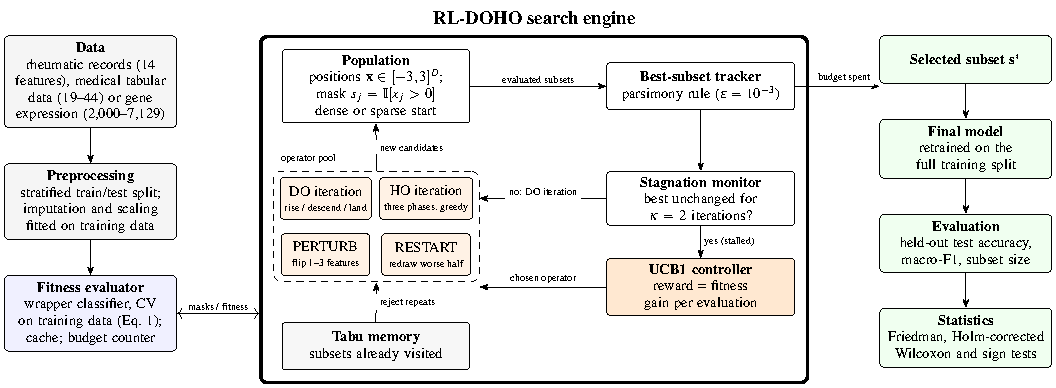
\includegraphics[width=\textwidth]{Fig1}
\caption{Architecture of the feature-selection pipeline. The data are split and preprocessed, and every candidate subset is scored by the wrapper fitness on the training data only, with a cache and a counter that enforces the evaluation budget. Inside the RL-DOHO engine, the population is updated by published DO iterations while the best subset improves. When the stagnation monitor detects $\kappa=2$ stalled iterations, the UCB1 controller chooses one operator from the pool, rewarded by the fitness gain per evaluation, and tabu memory rejects subsets already visited. When the budget is spent, the selected subset is used to retrain the final classifier, which is evaluated on held-out data.}
\label{fig:arch}
\end{figure}

Fig.~\ref{fig:arch} shows the overall pipeline; the components are described below.

\subsection{Problem formulation and budget}
A candidate solution is a binary mask $\mathbf{s}\in\{0,1\}^D$ over the $D$ available features, and $|\mathbf{s}|$ denotes how many of them are switched on. All methods are asked to minimize
\begin{equation}
f(\mathbf{s}) = \alpha\,\bigl(1-A_{\mathrm{CV}}(\mathbf{s})\bigr) + \beta\,\frac{|\mathbf{s}|}{D}, \qquad \alpha=0.99,\ \beta=0.01,
\label{eq:fitness}
\end{equation}
where $A_{\mathrm{CV}}$ is the cross-validated accuracy (balanced accuracy for GSE93272 and the five medical tabular datasets) of the wrapper classifier on the training data only, and $f=1$ for the empty mask. The fitness is deterministic for a given mask, so repeated masks are served from a cache. The budget $B$ is the same for all search methods and is counted in fitness calls; a call is charged to the budget even if its value is read from the cache. We count evaluations and not iterations because an HO iteration evaluates roughly three times as many candidates as a DO iteration, so equal iteration counts would not be a fair comparison.

\subsection{Encoding and initialization}
An agent is a point $\mathbf{x}\in[-3,3]^D$. Its mask is $s_j=\mathbb{I}[\sigma(x_j)>0.5]$ with $\sigma$ the logistic function, which simply means that feature $j$ is in the subset whenever $x_j>0$. With the \emph{dense} start, positions are drawn uniformly in $[-1,1]^D$, so each feature starts selected with probability 0.5. For the gene-expression data ($D>100$) all wrapper methods use a \emph{sparse} start instead. Here agent $i$ starts with a fraction $p_i$ of the features switched on, where $p_i$ is drawn log-uniformly between $\min(10/D,0.1)$ and $0.1$; the first subsets thus hold anything from about ten features up to a tenth of all of them. Selected coordinates are drawn from $\mathcal{U}(0.1,1)$ and the others from $\mathcal{U}(-1,-0.1)$.

\subsection{Published DO and HO update rules}
\emph{Dandelion Optimizer.} Following \citet{zhao2022do}, every DO iteration applies three stages to the whole population, with $t$ the iteration, $T$ the number of iterations the budget allows, $\mathbf{x}^\ast$ the elite and $\alpha=r\,(t^2/T^2-2t/T+1)$ with $r\sim\mathcal{U}(0,1)$. In the rising stage, with probability $P(\mathcal{N}(0,1)<1.5)\approx0.93$,
\begin{equation}
\mathbf{x}\leftarrow\mathbf{x}+\alpha\,v_xv_y\,\ln Y\,(\mathbf{x}_s-\mathbf{x}),
\end{equation}
where $\mathbf{x}_s$ is a random point in the search space, $v_x=r_\theta\cos\theta$, $v_y=r_\theta\sin\theta$, $r_\theta=e^{-\theta}$ with $\theta\sim\mathcal{U}(-\pi,\pi)$, and $\ln Y$ is the lognormal density evaluated at $|\mathcal{N}(0,1)|$. Otherwise the position is shrunk, $\mathbf{x}\leftarrow k\,\mathbf{x}$, with the schedule $k$ of \citet{zhao2022do}. In the descending stage, $\mathbf{x}\leftarrow\mathbf{x}-\alpha\boldsymbol{\beta}\odot(\bar{\mathbf{x}}-\alpha\boldsymbol{\beta}\odot\mathbf{x})$, with $\boldsymbol{\beta}\sim\mathcal{N}(0,1)^D$ and $\bar{\mathbf{x}}$ the population mean. In the landing stage,
\begin{equation}
\mathbf{x}\leftarrow\mathbf{x}^\ast+\mathrm{L\acute{e}vy}\odot\alpha\,(\mathbf{x}^\ast-\delta\,\mathbf{x}),\qquad \delta=2t/T,
\end{equation}
where the Lévy steps use exponent 1.5 and scale 0.01. A DO iteration therefore costs one evaluation per agent, i.e.\ $N$ in total.

\emph{Hippopotamus Optimization.} An HO iteration, as defined by \citet{amiri2024ho}, runs through three phases, and in each one a candidate is kept only if it improves on the agent it came from. In phase~1 (first half of the population), each agent generates a ``male'' candidate $\mathbf{x}+r(\mathbf{x}^{D}-I_1\mathbf{x})$ towards the dominant agent $\mathbf{x}^{D}$, and a ``female or immature'' candidate. Early in the run, as long as $e^{-t/T}>0.6$, this second candidate is placed relative to the mean $\mathbf{m}_G$ of a randomly chosen group of agents, as $\mathbf{x}+\mathbf{h}_1\odot(\mathbf{x}^{D}-I_2\mathbf{m}_G)$; later it is either $\mathbf{x}+\mathbf{h}_2\odot(\mathbf{m}_G-\mathbf{x}^{D})$ or a random point. The integers $I_1,I_2$ are 1 or 2 at random, and $\mathbf{h}$ is one of the five random vectors listed by \citet{amiri2024ho}. In phase~2 (second half), a random predator position is evaluated, and the agent jumps relative to it with a Lévy step (scale 0.05) and a distance-dependent term. Phase~3 applies to every agent and is a local move within bounds that narrow as $1/t$. With the predator points included, one HO iteration takes roughly $3N$ evaluations. The original papers leave some details open, such as the size of the random group behind $\mathbf{m}_G$, for which we draw a random size between 1 and $N$; our implementation is in the repository.

\subsection{RL-DOHO}
RL-DOHO (Fig.~\ref{fig:flow}, Algorithm~\ref{alg:rldoho}) uses plain DO iterations for as long as they keep improving the best subset. A stagnation counter $c$ counts consecutive iterations without an accepted change of the best subset. When $c$ reaches $\kappa=2$, a controller selects one of four arms for the next step:
\begin{itemize}
\item \textbf{PERTURB}: each agent in the worse half is replaced by a copy of the best position with $k\sim\mathcal{U}\{1,2,3\}$ randomly chosen features flipped. Each flipped coordinate is set to the opposite sign, with magnitude from $\mathcal{U}(0.5,2)$. This is a bit-flip local search around the best subset ($N/2$ evaluations).
\item \textbf{RESTART}: the worse half is replaced by fresh agents from the initial (dense or sparse) distribution, again $N/2$ evaluations. Unlike PERTURB, it moves the search away from the best subset.
\item \textbf{DO}: one more published DO iteration over all agents ($N$ evaluations), which amounts to carrying on as before.
\item \textbf{HO}: one published HO iteration, about $3N$ evaluations and so the most expensive arm.
\end{itemize}
PERTURB and RESTART draw candidates through a tabu memory that stores every subset the population has held during the run (HO's predator points are evaluated but not stored). A draw whose mask is already in the memory is redrawn, up to 20 times, after which the last draw is kept. The DO and HO schedules follow the fraction of the budget already spent, so that, for example, DO reaches its landing behaviour at the end of the budget whichever arms were used.

\emph{Controller.} The controller is a UCB1 bandit \citep{auer2002}. Each arm is pulled once in random order, and afterwards the arm
\begin{equation}
a_t=\arg\max_a\Bigl[\bar{Q}_a + \sqrt{\tfrac{2\ln N_t}{n_a}}\Bigr]
\end{equation}
is chosen, where $\bar{Q}_a$ is the mean reward of arm $a$, $n_a$ its pull count and $N_t=\sum_a n_a$. The reward of a pull is
\begin{equation}
r_t=0.8\,\min\!\Bigl(1,\frac{g_t}{g_{\max}}\Bigr)+0.2\,\frac{1}{|I_t|}\sum_{i\in I_t}\mathbb{I}\bigl[f_i<\tilde f_{t-1}\bigr],
\label{eq:reward}
\end{equation}
where $g_t$ is the decrease in the best fitness divided by the evaluations the step used, $g_{\max}$ is the largest such value observed so far in the run, $I_t$ is the set of agents the arm changed, and $\tilde f_{t-1}$ is the median fitness before the step. If a step merely swaps the best subset for a smaller one without lowering the best fitness, the gain part of its reward is zero. An earlier reward, 1 for any accepted change and otherwise the median term alone, is kept as an ablation.

\emph{Acceptance.} The parsimony rule from the earlier version is retained. The incumbent best is replaced when a candidate beats it by more than $\varepsilon=10^{-3}$ in fitness; inside that margin, the candidate wins if it has fewer features, or the same number and a lower fitness. In the clinical runs, where it was tested, this rule never changed an outcome (Section~\ref{sec:ablation}).

\emph{Q-learning controller (ablation).} To test whether a controller with state does better than the stateless bandit, we also ran RL-DOHO with tabular one-step Q-learning \citep{watkins1992}. The state combines the budget phase (first, middle or last third of the budget) with whether the previous intervention lowered the best fitness, giving six states. The actions are the four arms and the reward is (\ref{eq:reward}). Hyperparameters were a learning rate of 0.3, a discount of 0.5 and $\varepsilon$-greedy exploration with $\varepsilon=0.2$; the Q-table was initialised to zero for each run. These settings were fixed before the runs and not tuned.

\begin{figure}[t]
\centering
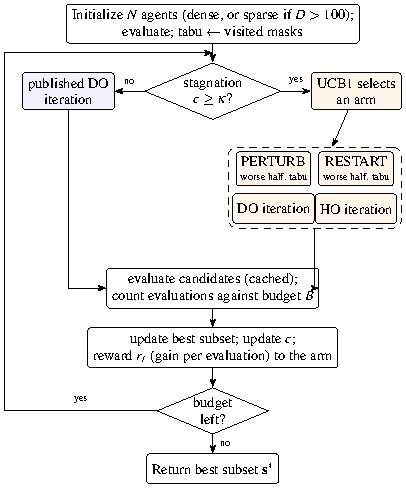
\includegraphics[width=0.62\textwidth]{Fig2}
\caption{Flow of one RL-DOHO run. Published DO iterations are used while the best subset improves; after $\kappa=2$ iterations without an accepted change, the UCB1 controller chooses one of four arms for the next step. The run stops when the evaluation budget is spent.}
\label{fig:flow}
\end{figure}

\begin{algorithm}[t]
\caption{RL-DOHO}\label{alg:rldoho}
\small
\begin{algorithmic}[1]
\Require population $N$, evaluation budget $B$, trigger $\kappa$
\State initialize positions (dense or sparse), evaluate, record best; tabu $\mathcal{T}\leftarrow$ visited masks; $c\leftarrow0$
\While{evaluations used $<B$}
  \If{$c<\kappa$} \State apply one published DO iteration to all agents
  \Else \State $a\leftarrow$ UCB1 choice among \{PERTURB, RESTART, DO, HO\}
    \If{$a\in$ \{PERTURB, RESTART\}} \State redraw the worse half with arm $a$, rejecting masks in $\mathcal{T}$
    \Else \State apply one published DO or HO iteration \EndIf
  \EndIf
  \State evaluate new candidates; add their masks to $\mathcal{T}$; update the best subset
  \State $c\leftarrow0$ if the best subset changed, else $c\leftarrow c+1$
  \If{an arm was pulled} \State give it reward $r_t$ from (\ref{eq:reward}) \EndIf
\EndWhile
\Ensure best mask $\mathbf{s}^\ast$
\end{algorithmic}
\end{algorithm}

\subsection{Fixed-switch hybrid (DOHO)}
DOHO is a control for the question of whether running both algorithms is already enough. It spends the first half of the evaluation budget on the published DO and the second half on the published HO. It has no stagnation trigger, local search, tabu memory or bandit.

\subsection{The intervention layer on other optimizers (GA+SI, HO+SI)}
To test whether the interventions help optimizers other than DO, we wrapped the same layer around the GA and around the published HO, which we call GA+SI and HO+SI (SI for stagnation-triggered interventions). GA+SI is in effect a memetic GA \citep{moscato1989}, a GA with a local search applied when it stalls, so it also serves as a memetic baseline. The base optimizer (GA or HO) is left alone while its best subset improves. After $\kappa=2$ stalled iterations, UCB1 with the gain reward chooses among PERTURB, RESTART and one iteration of the base optimizer, with the same tabu memory and acceptance rule as RL-DOHO. GA children are stored as positions $\pm1$ so that PERTURB and RESTART can act on them. An HO iteration costs about $3N$ evaluations and a GA generation $N$. Within one budget HO+SI therefore goes through roughly a third as many iterations as GA+SI, and has fewer chances to stall and trigger an intervention.



\section{Experimental Setup}\label{sec:setup}

\subsection{Datasets}
Table~\ref{tab:data} lists the datasets. The rheumatic dataset \citep{mahdi2025data} contains 12,085 records collected between 2019 and 2024 from one hospital and three diagnostic laboratories in Iraq. It has seven classes: rheumatoid arthritis (2,848), ankylosing spondylitis (2,127), Sj\"ogren's syndrome (1,852), psoriatic arthritis (1,783), no disease (1,604), systemic lupus erythematosus (1,355) and reactive arthritis (516). Its 14 features are age, gender, ESR, CRP, RF, anti-CCP, C3, C4, HLA-B27, ANA, anti-Ro, anti-La, anti-dsDNA and anti-Sm. Missing values are frequent, from 9\% (ESR) to 43\% (anti-Sm); age and gender are complete (Fig.~\ref{fig:eda}).

The four microarray datasets come from the scikit-feature repository \citep{li2017fs} and originate from colon tumour \citep{alon1999}, leukaemia \citep{golub1999}, lung carcinoma \citep{bhattacharjee2001} and glioma \citep{nutt2003} studies. GSE93272 is a whole-blood expression series from patients with rheumatoid arthritis and healthy controls \citep{tasaki2018}. Several of its 275 samples are repeat samples from the same individual, so we kept the first sample of each individual (101 people: 66 RA, 35 controls).

The five medical tabular datasets were taken from the PMLB collection \citep{olson2017pmlb}, which provides cleaned copies of UCI datasets. They cover breast tumour diagnosis from cell-nucleus features (WDBC, \citealp{street1993}; 357 benign, 212 malignant), hepatitis survival (Hepatitis; 123 and 32 patients), the differential diagnosis of six erythemato-squamous skin diseases (Dermatology, \citealp{guvenir1998}; 20--112 patients per class), cardiac SPECT images summarized as region-of-interest features (SPECTF, \citealp{kurgan2001}; 254 abnormal, 95 normal) and back-pain outcome (Backache; 155 and 25 patients). We chose them, before running any method on them, as openly available medical classification problems with 19--44 features, a range that lies between the clinical and the gene-expression data. Most of them are imbalanced (minority classes of 14--37\% in the binary ones), so these datasets and GSE93272 use balanced accuracy.

\begin{table}[t]
\centering
\caption{Datasets}
\label{tab:data}
\footnotesize
\setlength{\tabcolsep}{4pt}
\begin{tabular}{@{}lrrrl@{}}
\toprule
Dataset & Samples & Features & Classes & Test set \\
\midrule
Rheumatic \citep{mahdi2025data} & 12,085 & 14 & 7 & 2,417$^\ddagger$ \\
\midrule
Colon \citep{alon1999} & 62 & 2,000 & 2 & 19 (per seed) \\
ALL/AML \citep{golub1999} & 72 & 7,129 & 2 & 22 (per seed) \\
Lung \citep{bhattacharjee2001} & 203 & 3,312 & 5 & 61 (per seed) \\
Glioma \citep{nutt2003} & 50 & 4,434 & 4 & 15 (per seed) \\
GSE93272 \citep{tasaki2018} & 101 & 5,000$^\dagger$ & 2 & 31 (per seed) \\
\midrule
WDBC \citep{street1993} & 569 & 30 & 2 & 171 (per seed) \\
Hepatitis \citep{olson2017pmlb} & 155 & 19 & 2 & 47 (per seed) \\
Dermatology \citep{guvenir1998} & 366 & 34 & 6 & 110 (per seed) \\
SPECTF \citep{kurgan2001} & 349 & 44 & 2 & 105 (per seed) \\
Backache \citep{olson2017pmlb} & 180 & 32 & 2 & 54 (per seed) \\
\bottomrule
\multicolumn{5}{@{}l@{}}{\scriptsize $^\dagger$Most variable of 54,613 probes, chosen on each training split.}\\
\multicolumn{5}{@{}l@{}}{\scriptsize $^\ddagger$One fixed split for the main runs; two further splits in Section~\ref{sec:splits}.}
\end{tabular}
\end{table}

\begin{figure}[t]
\centering
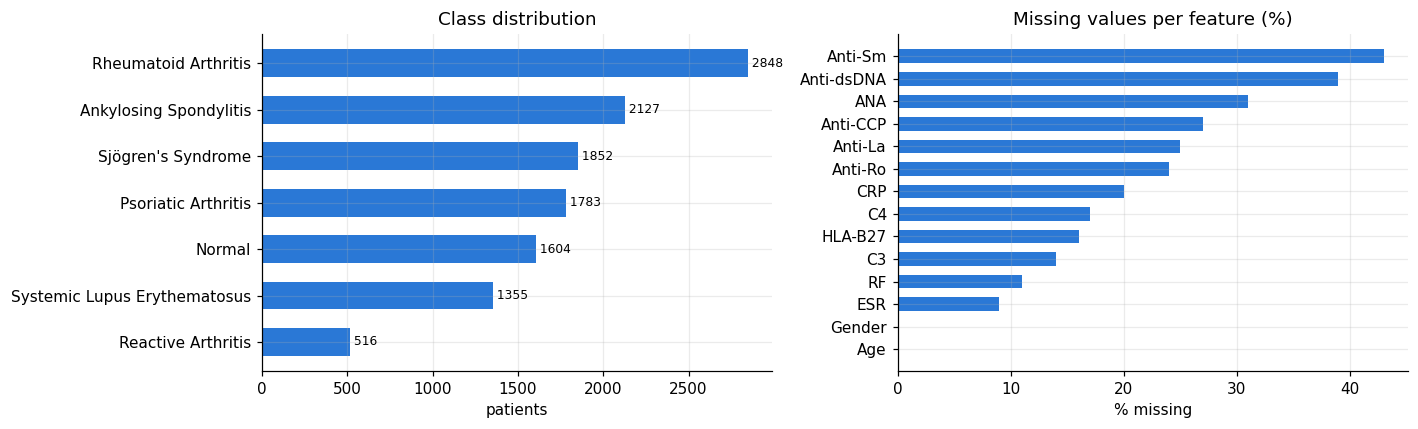
\includegraphics[width=0.85\textwidth]{Fig3}
\caption{Rheumatic and autoimmune disease dataset \citep{mahdi2025data}: class sizes (left) and percentage of missing values per variable before imputation (right). Classes range from 516 to 2,848 patients, and missingness from none (age, gender) to 43\% (anti-Sm).}
\label{fig:eda}
\end{figure}

\subsection{Protocols}
\emph{Rheumatic data.} A single stratified 80/20 split (9,668 training and 2,417 test patients) was used for the main runs, so the ten seeds vary only the search. Binary variables were encoded as 0/1. Mean imputation and standardization for numeric variables, and mode imputation for binary variables, were fitted on the training split only. The fitness used the mean 3-fold stratified cross-validated accuracy of an XGBoost \citep{chen2016xgb} and a histogram gradient-boosting classifier (60 trees, depth 4, learning rate 0.1), with SMOTE \citep{chawla2002} applied inside each training fold. Running both models on all 9,668 training patients for every candidate would have taken too long, so the fitness was computed on a fixed stratified subsample of 4,000 of them. For the final evaluation, both classifiers were retrained with 200 trees on the full training split, and we report their mean test accuracy and macro-F1. The population size was 12 and $B=252$. Seed 42 was used during development and was excluded; the evaluation uses seeds 0--9.

\emph{Repeated clinical splits.} To check that the clinical results do not depend on one split, we drew two further stratified 80/20 splits (random states 1 and 2). On each, the imputation, the scaling and the 4,000-patient fitness subsample were refitted on that split's training data, and every method was run with seeds 0--4. Together with seeds 0--4 of the main runs this gives 3 splits $\times$ 5 seeds = 15 paired runs per method. Our original plan was four new splits. Each one needs roughly an hour of fresh fitness evaluations on our hardware, so we cut the number to two, and we made that decision before any of the new splits had finished running.

\emph{Gene-expression and medical tabular data.} For each seed, a new stratified 70/30 split was drawn and min-max scaling was fitted on the training part. The fitness used the 5-fold cross-validated accuracy (balanced accuracy for GSE93272 and the tabular datasets) of a 5-nearest-neighbour classifier on the training part, and the test score is that of the same classifier retrained on the training part. For GSE93272, the 5,000 most variable probes were selected on each training split before the search. Population size and budget were 20 and $B=1{,}020$. The gene-expression runs used the sparse start and the tabular runs the dense start ($D<100$).

\emph{Second classifier.} After the main results, we repeated the tabular benchmark with a support vector machine (RBF kernel, $C=1$, $\gamma$ set by scikit-learn's \texttt{scale} rule, untuned) in place of 5-NN, in both the fitness and the test evaluation, with the same splits, seeds and budgets. Every wrapper and filter method, the two add-ons and PERTURB alone were rerun.

\subsection{Baselines}
The wrapper baselines use the fitness (\ref{eq:fitness}) and the budget described above. The GA, binary PSO and binary GWO use the same initial population as the other methods. Our GA is a standard binary one: tournament size 3, uniform crossover applied with probability 0.9, per-bit mutation probability $1/D$, and one elite carried over. Binary PSO \citep{kennedy1997} uses sigmoid velocity transfer, $c_1=c_2=2$, velocity clamp 6 and inertia decreasing from 0.9 to 0.4; with the sparse start, its initial velocities are set consistent with the initial masks. Binary GWO \citep{mirjalili2014gwo,emary2016bgwo} updates continuous positions and binarizes them with the same rule as DO and HO. On the rheumatic data the GA, PSO, GWO and filter results of the main runs come from the earlier runs of this study, which used the same fitness, split, seeds and budget.

The three non-wrapper methods rank features on the same training data used by the fitness. LASSO uses the absolute coefficients of an L1-penalized logistic regression \citep{tibshirani1996} on standardized data ($C=0.5$). mRMR \citep{peng2005} uses mutual information minus mean absolute correlation with the already selected features, chosen greedily for up to 2,000 features, with the remainder ordered by relevance. ReliefF \citep{kononenko1994} was run with 500 sampled instances and 10 neighbours. For each ranking, the number of retained features $k$ is the one that minimizes the fitness (\ref{eq:fitness}), searched over all $k\le D$ when $D\le40$ and over $k\in\{5,10,20,50,100,200,500,1000,2000,D\}$ otherwise. No test data is used to choose $k$. The full feature set is included as a reference.

\subsection{Hypotheses fixed in advance}
The first four hypotheses, and the tests for them, were set down before the main experiments:
\begin{itemize}
\item \textbf{H1}: RL-DOHO ends with lower fitness than the published DO.
\item \textbf{H2}: RL-DOHO against the published HO, with no direction predicted.
\item \textbf{H3}: given three times the budget, RL-DOHO with its UCB controller and gain reward ends with lower fitness than the same method choosing arms at random.
\item \textbf{H4}: on gene data, the sparse start gives RL-DOHO lower fitness than the dense start.
\end{itemize}
H1--H3 were tested on the clinical and gene-expression datasets and H4 on the five gene-expression datasets, each with a two-sided sign test over the paired runs.

H5--H8 came later. They were formulated once H1--H4 had been tested, but before any of the extension runs (tabular datasets, add-ons, Q-learning controller, $\kappa$ sweep, repeated splits):
\begin{itemize}
\item \textbf{H5}: at $3\times$ budget, Q-learning versus random arm selection (two-sided, no predicted direction).
\item \textbf{H6}: GA+SI reaches lower fitness than the GA, and HO+SI lower than HO (Holm-corrected over the two).
\item \textbf{H7} (null): RL-DOHO's fitness does not depend on $\kappa\in\{1,2,3,4\}$; Friedman test.
\item \textbf{H8}: on the repeated clinical splits, RL-DOHO against each other method, with no direction predicted.
\end{itemize}
H5--H7 were tested on all eleven datasets. Before the SVM runs we fixed a ninth:
\begin{itemize}
\item \textbf{H9}: with an SVM, the tabular findings replicate: RL-DOHO beats DO (H9a); RL-DOHO against HO (H9b), the GA against RL-DOHO (H9c) and RL-DOHO against PERTURB alone (H9e) with no direction predicted; HO+SI beats HO, and GA+SI against the GA with no direction predicted (H9d).
\end{itemize}
After the main and extension results were known, we fixed a tenth, aimed at the controller result:
\begin{itemize}
\item \textbf{H10a}: at three times the budget, UCB1 started from the statistics of two earlier runs on the same training data reaches lower fitness than random arm selection (ten KNN datasets, two-sided sign test).
\end{itemize}
Three further extensions were specified at the same time (Section~S3 of Online Resource~1) but were not run. After the H10a diagnostics we fixed two more:
\begin{itemize}
\item \textbf{H11a/b}: at three times the budget, UCB1 with a reward that credits only improvement of the best subset reaches lower fitness than random arm selection, with the default exploration constant (H11a) and with $c=0.2$ (H11b), Holm-corrected over the two.
\end{itemize}
Finally, to test whether DO is weak only because of the binary encoding, we fixed:
\begin{itemize}
\item \textbf{H12a--d}: at the standard budget on the ten KNN datasets, RL-DOHO against DO with a 10$\times$ (H12a) and 100$\times$ (H12b) larger landing-stage L\'evy step and against DO with the standard stochastic sigmoid transfer function \citep{kennedy1997,mirjalili2013sv} (H12c); and RL-DOHO against DO when both use the 100$\times$ step (H12d). Holm-corrected over the four.
\end{itemize}
All other settings of RL-DOHO ($\varepsilon$, the reward weights, the UCB constant, the number of flipped features, the tabu redraws) were carried over unchanged from the earlier version of this study and were not tuned.

\subsection{Statistical analysis}
The statistics are nonparametric, as recommended by \citet{demsar2006}:
\begin{itemize}
\item \textbf{Within each dataset:} the 11 methods are compared over the 10 seeds with a Friedman test \citep{friedman1937}. RL-DOHO is compared with each other method by a Wilcoxon signed-rank test \citep{wilcoxon1945}, with zero differences split between the two sides and a Holm correction \citep{holm1979} over the ten comparisons.
\item \textbf{Across datasets:} paired runs from all datasets are pooled, and wins against losses are tested with a two-sided sign test (Holm correction over the ten comparisons for each metric). These pooled tests treat the runs as independent although runs on the same dataset share data, so the dataset-level analysis below, with one observation per dataset, is the conservative check.
\item \textbf{Dataset-level view:} each method's mean on a dataset gives one rank per dataset; these ranks go into a Friedman test and a Nemenyi critical-difference analysis \citep{nemenyi1963}, where 11 datasets and 11 methods give a critical difference of 4.55 rank units.
\end{itemize}
Ablation comparisons report unadjusted sign-test $p$-values, as exploratory results. Differences smaller than $10^{-12}$ count as ties.


\subsection{Use of generative AI}
Generative AI (Claude, Anthropic) was used to help write and debug the experiment and analysis code, to suggest analyses, and to draft and edit parts of the manuscript text. The authors ran all experiments, reviewed the code and the text, checked every reported number against the per-run results in the public repository, and take full responsibility for the content of this article.

\section{Results}\label{sec:results}

\subsection{Rheumatic and autoimmune disease data}
Table~\ref{tab:rheum} and Fig.~\ref{fig:rheumbox} summarize the clinical results. Except for DO, the boxes for fitness and test accuracy in the figure overlap heavily; subset size is the panel that separates the methods.
\begin{itemize}
\item \textbf{Within the DO--HO family}, RL-DOHO had the lowest mean fitness: 0.1832, against 0.1838 for HO, 0.1857 for DOHO and 0.2280 for DO.
\item \textbf{Against DO}, RL-DOHO was better in all ten runs on fitness, test accuracy and macro-F1 (Holm $p=0.020$ each).
\item \textbf{Against HO} (5/2/3) and DOHO (8/0/2; unadjusted $p=0.020$, Holm $p=0.12$), the fitness differences were not significant after correction.
\item \textbf{The GA and binary PSO reached lower fitness} (0.1821 and 0.1828), and RL-DOHO ranked third of 11. The GA found the best subset seen in any run (fitness 0.18200, 10 features) in 7 of 10 runs, BPSO in 4, and RL-DOHO and BGWO in one each.
\item \textbf{Against the filters}, RL-DOHO's fitness was lower than LASSO's and ReliefF's in all ten runs (Holm $p=0.020$ each). On test accuracy, however, ReliefF (84.97\%) and LASSO (84.92\%) were ahead of RL-DOHO (84.33\%) in all ten runs (Holm $p=0.020$). With a fixed split, LASSO is deterministic here and ReliefF nearly so, so this paired test mostly reflects RL-DOHO's run-to-run variation.
\item \textbf{Test accuracy range}: apart from DO (79.99\%), all methods fall between 83.85\% and 84.97\%, a range of about 27 of the 2,417 test patients.
\end{itemize}

\begin{table}[t]
\centering
\caption{Rheumatic and autoimmune disease data: mean $\pm$ standard deviation over ten seeds, at a budget of 252 fitness evaluations. CV and test accuracy and macro-F1 in \%. Ranks are averaged over seeds (1 = best). Best value per column in bold.}
\label{tab:rheum}
\footnotesize
\setlength{\tabcolsep}{5pt}
\begin{tabular}{@{}lccccccc@{}}
\toprule
Method & Fitness & CV acc. & Test acc. & Test macro-F1 & Features & Rank (fitness) & Rank (test acc.) \\
\midrule
\textbf{RL-DOHO} & 0.1832 $\pm$ 0.0013 & \textbf{82.38} & 84.33 $\pm$ 0.42 & 83.96 & 12.2 & 3.50 & 6.70 \\
DO & 0.2280 $\pm$ 0.0273 & 77.63 & 79.99 $\pm$ 3.08 & 79.66 & \textbf{9.1} & 10.95 & 10.95 \\
HO & 0.1838 $\pm$ 0.0013 & 82.34 & 84.29 $\pm$ 0.09 & 83.88 & 12.6 & 4.30 & 7.00 \\
DOHO & 0.1857 $\pm$ 0.0022 & 82.16 & 84.45 $\pm$ 0.30 & 84.01 & 12.7 & 6.75 & 5.75 \\
\midrule
GA & \textbf{0.1821} $\pm$ 0.0002 & 82.36 & 84.45 $\pm$ 0.35 & 83.86 & 10.4 & \textbf{1.60} & 5.50 \\
BPSO & 0.1828 $\pm$ 0.0010 & 82.33 & 84.54 $\pm$ 0.32 & 84.06 & 11.0 & 3.00 & 5.50 \\
BGWO & 0.1894 $\pm$ 0.0116 & 81.62 & 83.85 $\pm$ 1.30 & 83.28 & 10.4 & 6.60 & 6.90 \\
\midrule
LASSO & 0.1868 $\pm$ 0.0000 & 82.00 & 84.92 $\pm$ 0.00 & \textbf{84.81} & 12.0 & 7.80 & 2.10 \\
mRMR & 0.1848 $\pm$ 0.0021 & 82.19 & 84.51 $\pm$ 0.45 & 84.15 & 11.9 & 5.50 & 5.40 \\
ReliefF & 0.1854 $\pm$ 0.0012 & 82.10 & \textbf{84.97} $\pm$ 0.04 & 84.76 & 11.4 & 6.40 & \textbf{1.40} \\
All features & 0.1884 $\pm$ 0.0000 & 81.98 & 83.97 $\pm$ 0.00 & 83.50 & 14.0 & 9.60 & 8.80 \\
\bottomrule
\end{tabular}
\end{table}

\begin{figure}[t]
\centering
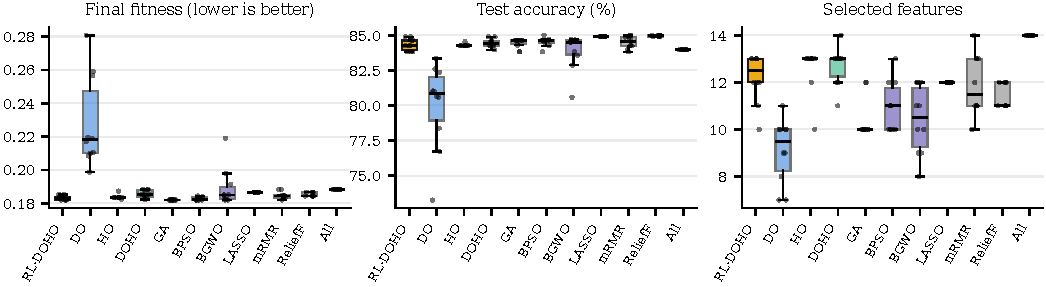
\includegraphics[width=\textwidth]{Fig4}
\caption{Rheumatic data: distribution over ten seeds of final fitness, test accuracy and subset size for every method (dots are individual runs; ``All'' is the full feature set). Apart from DO, the methods differ far more in subset size than in fitness or test accuracy.}
\label{fig:rheumbox}
\end{figure}

Fig.~\ref{fig:convrheum} shows why DO fares so poorly on this problem. The published DO improved on the best subset of its initial population in only 1 of the 10 runs. The reason lies in the landing stage. It puts every agent within a small Lévy step of the elite, so after the first iteration almost no coordinate changes sign, and the population produces the elite's subset over and over. HO's greedy, randomized phases do not have this problem, and RL-DOHO escapes it through its interventions. Here, in fact, RL-DOHO's own DO steps never lowered the best fitness at all; the HO arm accounts for 80\% of its total improvement (Table~\ref{tab:arms}).

\begin{figure}[t]
\centering
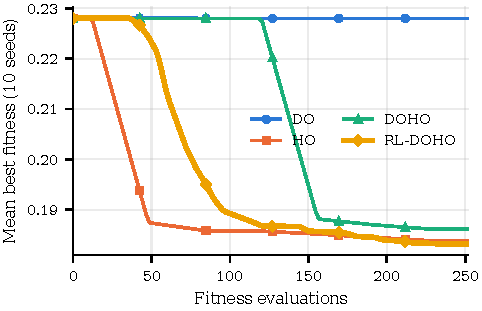
\includegraphics[width=0.62\textwidth]{Fig5}
\caption{Mean best fitness against fitness evaluations used, over ten seeds, on the rheumatic data for the DO--HO family. DO's curve stays almost flat after its first iteration, while HO and RL-DOHO keep improving.}
\label{fig:convrheum}
\end{figure}

The selected variables were similar across the wrapper methods (Fig.~\ref{fig:freq}). RL-DOHO kept ESR, CRP, RF, anti-CCP, C3, C4, gender, ANA, anti-Ro and anti-La in every run and HLA-B27 in nine. It kept anti-dsDNA in two runs and anti-Sm in three: these are the two variables with the most missing values. The GA, which reached the lowest fitness, also dropped anti-dsDNA and anti-Sm and, unlike RL-DOHO, usually dropped age and HLA-B27. LASSO and ReliefF kept HLA-B27, anti-dsDNA (LASSO) and anti-Sm, and dropped age and gender.

\begin{figure}[t]
\centering
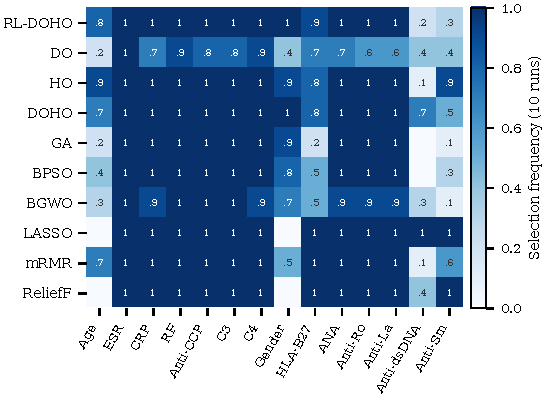
\includegraphics[width=0.62\textwidth]{Fig6}
\caption{Rheumatic data: fraction of the ten runs in which each method selected each variable (blank = never). Most wrappers keep the inflammatory markers and the common autoantibodies, and drop anti-dsDNA and anti-Sm, the two variables with the most missing values.}
\label{fig:freq}
\end{figure}

This comparison uses a single train/test split. Section~\ref{sec:splits} repeats it on two further splits.

\subsection{Gene-expression data}
Table~\ref{tab:genes} and Fig.~\ref{fig:convgenes} give the results on the five gene-expression datasets. On all five datasets DO's curve levels off early and finishes above the others, whereas HO and RL-DOHO are still improving when the budget runs out.
\begin{itemize}
\item \textbf{Against DO}, RL-DOHO reached lower fitness on all five datasets; the per-dataset difference was significant after correction on Colon, ALL/AML and Lung.
\item \textbf{Against HO}, its mean fitness was lower on Colon, ALL/AML and Glioma and higher on Lung and GSE93272, with no significant per-dataset difference; on ALL/AML HO was ahead in more runs (5 against 4).
\item \textbf{The GA} had the lowest wrapper fitness on four of the five datasets; RL-DOHO had it on ALL/AML.
\item \textbf{Binary PSO and GWO} kept many more genes than the other wrappers (240--1,280 on average, against 40--330), probably because their position updates drift away from the sparse initial masks.
\end{itemize}

\begin{table}[t]
\centering
\caption{Gene-expression datasets: mean fitness, mean test accuracy (\%, balanced accuracy for GSE93272) and mean number of selected features ($|S|$) over ten seeds, each with its own train/test split, at a budget of 1,020 fitness evaluations. All wrapper methods start from the sparse initial population. Best value per column in bold.}
\label{tab:genes}
\footnotesize
\setlength{\tabcolsep}{3.2pt}
\begin{tabular}{@{}l ccc ccc ccc ccc ccc@{}}
\toprule
& \multicolumn{3}{c}{Colon} & \multicolumn{3}{c}{ALL/AML} & \multicolumn{3}{c}{Lung} & \multicolumn{3}{c}{Glioma} & \multicolumn{3}{c}{GSE93272} \\
\cmidrule(lr){2-4}\cmidrule(lr){5-7}\cmidrule(lr){8-10}\cmidrule(lr){11-13}\cmidrule(l){14-16}
Method & Fit. & Acc. & $|S|$ & Fit. & Acc. & $|S|$ & Fit. & Acc. & $|S|$ & Fit. & Acc. & $|S|$ & Fit. & Acc. & $|S|$ \\
\midrule
\textbf{RL-DOHO} & 0.083 & 73.7 & 58 & 0.052 & 83.2 & 63 & 0.034 & 93.3 & 231 & 0.145 & 78.7 & 333 & 0.079 & 87.1 & 100 \\
DO & 0.127 & 71.1 & 70 & 0.105 & 80.5 & 115 & 0.045 & 94.4 & 217 & 0.184 & 75.3 & 69 & 0.095 & 84.9 & 148 \\
HO & 0.090 & 71.1 & 63 & 0.059 & 80.0 & 43 & 0.033 & 93.3 & 241 & 0.153 & 76.7 & 63 & 0.073 & 88.1 & 82 \\
DOHO & 0.111 & 71.1 & 64 & 0.079 & 80.9 & 61 & 0.036 & 93.8 & 226 & 0.170 & 78.7 & 85 & 0.087 & 85.8 & 142 \\
\midrule
GA & 0.062 & 76.3 & 62 & 0.054 & 83.6 & 150 & 0.028 & 93.3 & 162 & 0.111 & 76.7 & 91 & 0.053 & 87.4 & 141 \\
BPSO & 0.137 & 73.7 & 239 & 0.112 & 82.3 & 950 & 0.037 & 94.4 & 590 & 0.197 & 80.0 & 628 & 0.113 & 87.4 & 941 \\
BGWO & 0.100 & 75.3 & 390 & 0.093 & 82.7 & 1278 & 0.034 & 93.6 & 611 & 0.188 & 81.3 & 558 & 0.092 & 86.5 & 1025 \\
\midrule
LASSO & \textbf{0.028} & \textbf{82.1} & \textbf{16} & \textbf{0.008} & 91.4 & \textbf{33} & \textbf{0.019} & 94.4 & \textbf{77} & \textbf{0.009} & 67.3 & \textbf{18} & \textbf{0.004} & 88.9 & \textbf{48} \\
mRMR & 0.104 & 80.0 & 83 & 0.012 & \textbf{94.1} & 110 & 0.024 & \textbf{95.1} & 170 & 0.119 & 77.3 & 86 & 0.061 & \textbf{89.4} & 182 \\
ReliefF & 0.093 & 77.9 & 41 & 0.036 & 92.7 & 57 & 0.044 & 93.6 & 645 & 0.150 & 75.3 & 64 & 0.093 & 82.8 & 115 \\
All features & 0.260 & 72.6 & 2000 & 0.212 & 82.3 & 7129 & 0.067 & 94.3 & 3312 & 0.299 & \textbf{84.0} & 4434 & 0.191 & 85.3 & 5000 \\
\bottomrule
\end{tabular}
\end{table}

\begin{figure}[t]
\centering
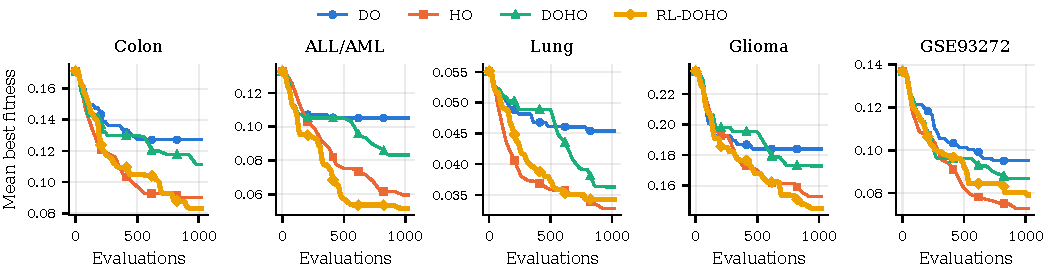
\includegraphics[width=\textwidth]{Fig7}
\caption{Mean best fitness against fitness evaluations, over ten seeds, on the gene-expression datasets for the DO--HO family (20 agents, 1,020 evaluations).}
\label{fig:convgenes}
\end{figure}

The filter methods behaved as in earlier work. LASSO reached the lowest fitness on every dataset, using 16--77 genes on average. mRMR had lower mean fitness than RL-DOHO on four of the five datasets, significantly so on ALL/AML and Lung. RL-DOHO reached lower fitness than ReliefF on Lung (Holm $p=0.035$). On held-out data the picture changes:
\begin{itemize}
\item Only two per-dataset test-accuracy differences between RL-DOHO and a filter were significant: mRMR and ReliefF were ahead on ALL/AML (Holm $p=0.039$).
\item On Glioma, LASSO had the best fitness (0.0085) but the lowest test accuracy (67.3\% against 78.7\% for RL-DOHO). RL-DOHO's macro-F1 was higher in all ten runs (Holm $p=0.020$).
\item Test sets here have only 15--61 samples per split, and one misclassification shifts accuracy by 1.6--6.7 points, which limits how much these accuracies can show.
\end{itemize}
Test accuracy is plotted against subset size in Fig.~\ref{fig:size}. Subset sizes span more than two orders of magnitude, from tens of genes to the full set, yet no method is the most accurate on all five datasets, so keeping fewer genes did not systematically cost accuracy.

\begin{figure}[t]
\centering
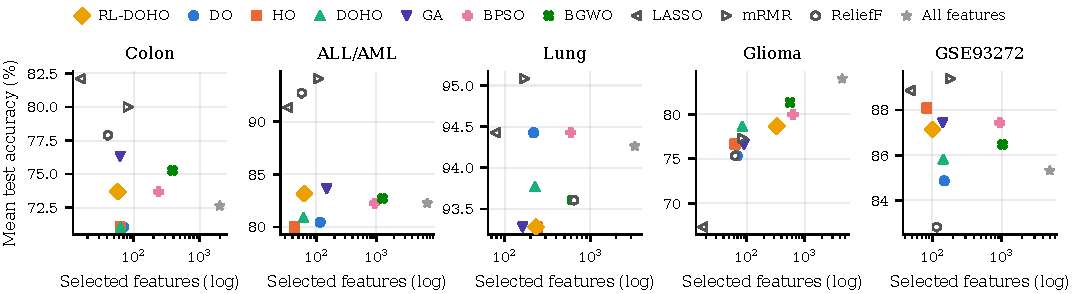
\includegraphics[width=\textwidth]{Fig8}
\caption{Mean test accuracy against mean number of selected features (log scale) on the gene-expression datasets. Hollow markers are filter or embedded methods.}
\label{fig:size}
\end{figure}


\subsection{Medical tabular datasets}
Table~\ref{tab:tab} gives the results on the five medical tabular datasets.
\begin{itemize}
\item \textbf{Against DO}, RL-DOHO reached lower fitness in 49 of 50 runs, significantly so on every dataset after correction.
\item \textbf{Against HO} it was ahead in 30 runs and behind in 20 (Holm $p=0.61$), with no significant per-dataset difference; against the fixed hybrid it was ahead in 35 and behind in 15 (Holm $p=0.026$).
\item \textbf{The GA} reached lower fitness than RL-DOHO in 45 of the 50 runs and on every dataset, significantly so on four of the five. Binary PSO and GWO were level with RL-DOHO (each ahead in 30 runs and behind in 20, Holm $p=0.61$).
\item \textbf{Against the filters}, RL-DOHO reached lower fitness than mRMR and ReliefF in 48 of 50 runs and than LASSO in 38 (all Holm $p\le0.002$). Unlike on gene data, the filters did not lead on fitness here.
\item \textbf{Test scores:} the per-dataset Friedman test on test balanced accuracy was not significant on any of the five datasets ($p=0.21$--$0.97$), and no pooled test-accuracy or macro-F1 comparison was significant after correction.
\item \textbf{Backache and Hepatitis are difficult for 5-NN.} Averaged over the 11 methods, test balanced accuracy was 53.6\% on Backache and 63.7\% on Hepatitis, and their test sets hold only about 8 and 10 minority-class patients. With so few minority cases, fitness gaps on these two datasets are a weak guide to held-out performance, so Section~\ref{sec:pooled} repeats the main comparisons without them.
\end{itemize}
Over the 50 tabular runs RL-DOHO had an average per-run fitness rank of 4.15 among the 11 methods, behind the GA (1.82), binary PSO (3.28) and binary GWO (3.29), and ahead of HO (4.75).

\begin{table}[t]
\centering
\caption{Medical tabular datasets: mean fitness, mean test balanced accuracy (\%) and mean number of selected features ($|S|$) over ten seeds, each with its own train/test split, at a budget of 1,020 fitness evaluations. All wrapper methods start from the dense initial population. Best value per column in bold.}
\label{tab:tab}
\footnotesize
\setlength{\tabcolsep}{3.2pt}
\begin{tabular}{@{}l ccc ccc ccc ccc ccc@{}}
\toprule
& \multicolumn{3}{c}{WDBC} & \multicolumn{3}{c}{Hepatitis} & \multicolumn{3}{c}{Dermatology} & \multicolumn{3}{c}{SPECTF} & \multicolumn{3}{c}{Backache} \\
\cmidrule(lr){2-4}\cmidrule(lr){5-7}\cmidrule(lr){8-10}\cmidrule(lr){11-13}\cmidrule(l){14-16}
Method & Fit. & Acc. & $|S|$ & Fit. & Acc. & $|S|$ & Fit. & Acc. & $|S|$ & Fit. & Acc. & $|S|$ & Fit. & Acc. & $|S|$ \\
\midrule
\textbf{RL-DOHO} & 0.029 & 94.3 & 13 & 0.209 & 64.2 & \textbf{7} & 0.025 & 95.0 & 17 & 0.167 & 73.1 & 22 & 0.316 & 54.3 & 10 \\
DO & 0.041 & 94.2 & 16 & 0.269 & 64.6 & 9 & 0.050 & 94.3 & 18 & 0.225 & 73.8 & 23 & 0.388 & 53.3 & 17 \\
HO & 0.032 & 94.5 & 13 & 0.221 & 62.1 & 7 & 0.026 & 95.4 & 24 & 0.178 & 73.7 & 18 & 0.310 & 53.8 & 12 \\
DOHO & 0.034 & 94.6 & 14 & 0.219 & 63.4 & 7 & 0.030 & 96.0 & 25 & 0.190 & 71.1 & 19 & 0.325 & 54.3 & 13 \\
\midrule
GA & \textbf{0.025} & 94.7 & 14 & 0.198 & 66.3 & 8 & \textbf{0.016} & 95.6 & \textbf{16} & \textbf{0.131} & 75.3 & 21 & \textbf{0.284} & 54.2 & 12 \\
BPSO & 0.029 & 95.2 & 15 & \textbf{0.189} & 61.7 & 8 & 0.020 & 95.2 & 20 & 0.172 & \textbf{75.8} & 22 & 0.297 & 52.6 & 14 \\
BGWO & 0.028 & 94.5 & 14 & 0.221 & \textbf{66.4} & 8 & 0.019 & 95.8 & 19 & 0.156 & 75.5 & 24 & 0.300 & 53.7 & 13 \\
\midrule
LASSO & 0.033 & 94.8 & \textbf{11} & 0.249 & 63.6 & 9 & 0.026 & 96.0 & 18 & 0.214 & 73.1 & \textbf{11} & 0.367 & 53.1 & \textbf{9} \\
mRMR & 0.036 & 94.5 & 13 & 0.251 & 62.4 & 8 & 0.039 & \textbf{96.1} & 23 & 0.285 & 68.9 & 23 & 0.382 & 53.4 & 14 \\
ReliefF & 0.036 & 94.0 & 12 & 0.264 & 59.9 & 8 & 0.039 & 95.7 & 30 & 0.238 & 74.3 & 15 & 0.387 & 52.7 & 13 \\
All features & 0.053 & \textbf{95.3} & 30 & 0.323 & 65.7 & 19 & 0.059 & 95.2 & 34 & 0.314 & 70.7 & 44 & 0.433 & \textbf{54.4} & 32 \\
\bottomrule
\end{tabular}
\end{table}

\subsection{Comparison across all eleven datasets}\label{sec:pooled}
Table~\ref{tab:pooled} pools the 110 paired runs.
\begin{itemize}
\item \textbf{Fitness, against the other wrapper methods:} RL-DOHO was ahead of DO in 103 runs and behind in 4, ahead of DOHO in 81 and behind in 28, and ahead of binary PSO in 70 and behind in 38. All three differences are significant after correction. Against binary GWO it was ahead in 67 runs and behind in 43 (Holm $p=0.084$).
\item \textbf{Against HO}, it was level (58 against 49, Holm $p=0.59$).
\item \textbf{The GA} reached lower fitness significantly more often (85 against 22, Holm $p<0.001$).
\item \textbf{Against the filters}, RL-DOHO was ahead of ReliefF (84 against 26) and mRMR (68 against 40) after correction and level with LASSO (49 against 61), which led on gene data and trailed on the other two data types.
\item \textbf{Test accuracy:} no comparison was significant after correction. On macro-F1, LASSO was ahead of RL-DOHO (66 against 36, Holm $p=0.039$).
\end{itemize}
Restricted to the six datasets of the main study (60 runs), the figures are those of the earlier analysis: ahead of DO 54 against 3, level with HO 28 against 29, behind the GA 18 against 40.

\emph{Sensitivity to the two weakest datasets.} Table~\ref{tab:weak} repeats the main comparisons without Backache and Hepatitis (90 runs). The conclusions about DO, HO, the GA, the fixed hybrid, binary PSO, the add-ons, the controllers and $\kappa$ are unchanged. One result does not survive: RL-DOHO's lead over mRMR (48 against 40, $p=0.46$). The advantage of PERTURB alone over the full arm set also becomes non-significant over the remaining 90 runs (47 against 37, $p=0.33$), but only because those runs are dominated by the gene data, where PERTURB alone is behind; on the three remaining tabular datasets it is still ahead (22 against 5, $p=0.002$).

\begin{table}[t]
\centering
\caption{Main comparisons with and without the two weakest datasets (Backache and Hepatitis): W/T/L for the first-named method on fitness and unadjusted two-sided sign-test $p$.}
\label{tab:weak}
\footnotesize
\setlength{\tabcolsep}{2.4pt}
\begin{tabular}{@{}lcccc@{}}
\toprule
& \multicolumn{2}{c}{All 11 datasets} & \multicolumn{2}{c}{Without the two} \\
\cmidrule(lr){2-3}\cmidrule(l){4-5}
Comparison & W/T/L & $p$ & W/T/L & $p$ \\
\midrule
RL-DOHO vs.\ DO & 103/3/4 & $<$0.001 & 83/3/4 & $<$0.001 \\
RL-DOHO vs.\ HO & 58/3/49 & 0.439 & 47/3/40 & 0.520 \\
RL-DOHO vs.\ DOHO & 81/1/28 & $<$0.001 & 69/1/20 & $<$0.001 \\
RL-DOHO vs.\ GA & 22/3/85 & $<$0.001 & 19/2/69 & $<$0.001 \\
RL-DOHO vs.\ BPSO & 70/2/38 & 0.003 & 64/2/24 & $<$0.001 \\
RL-DOHO vs.\ mRMR & 68/2/40 & 0.009 & 48/2/40 & 0.456 \\
HO+SI vs.\ HO & 71/10/29 & $<$0.001 & 54/8/28 & 0.005 \\
GA+SI vs.\ GA & 45/16/49 & 0.757 & 36/10/44 & 0.434 \\
PERTURB only vs.\ RL-DOHO & 64/6/40 & 0.024 & 47/6/37 & 0.326 \\
Q-learning vs.\ random arm, 3$\times$ & 46/8/56 & 0.373 & 37/7/46 & 0.380 \\
$\kappa\in\{1,2,3,4\}$ (Friedman) & -- & $<$0.001 & -- & $<$0.001 \\
\bottomrule
\end{tabular}
\end{table}

\begin{table}[t]
\centering
\caption{RL-DOHO against each method over all 110 paired runs (11 datasets $\times$ 10 seeds): wins/ties/losses for RL-DOHO and Holm-adjusted sign-test $p$-values. Bold: $p<0.05$.}
\label{tab:pooled}
\footnotesize
\setlength{\tabcolsep}{2.6pt}
\begin{tabular}{@{}lcccccc@{}}
\toprule
& \multicolumn{2}{c}{Fitness} & \multicolumn{2}{c}{Test accuracy} & \multicolumn{2}{c}{Macro-F1} \\
\cmidrule(lr){2-3}\cmidrule(lr){4-5}\cmidrule(l){6-7}
vs. & W/T/L & $p$ & W/T/L & $p$ & W/T/L & $p$ \\
\midrule
DO & 103/3/4 & \textbf{$<$0.001} & 58/14/38 & 0.467 & 57/8/45 & 1.000 \\
HO & 58/3/49 & 0.588 & 52/12/46 & 1.000 & 55/7/48 & 1.000 \\
DOHO & 81/1/28 & \textbf{$<$0.001} & 44/13/53 & 1.000 & 47/7/56 & 1.000 \\
\midrule
GA & 22/3/85 & \textbf{$<$0.001} & 48/14/48 & 1.000 & 52/11/47 & 1.000 \\
BPSO & 70/2/38 & \textbf{0.013} & 49/14/47 & 1.000 & 51/10/49 & 1.000 \\
BGWO & 67/0/43 & 0.084 & 43/12/55 & 1.000 & 44/7/59 & 1.000 \\
\midrule
LASSO & 49/0/61 & 0.588 & 36/11/63 & 0.086 & 36/8/66 & \textbf{0.039} \\
mRMR & 68/2/40 & \textbf{0.036} & 41/11/58 & 0.751 & 42/9/59 & 0.887 \\
ReliefF & 84/0/26 & \textbf{$<$0.001} & 41/10/59 & 0.709 & 42/7/61 & 0.681 \\
All features & 110/0/0 & \textbf{$<$0.001} & 44/14/52 & 1.000 & 45/10/55 & 1.000 \\
\bottomrule
\end{tabular}
\end{table}

Fig.~\ref{fig:cd} ranks the methods by their mean on each dataset.
\begin{itemize}
\item \textbf{Fitness:} the dataset-level Friedman test is significant ($\chi^2=62.99$, $p<0.001$). The GA (1.91) ranks first and RL-DOHO second (4.00), followed by LASSO (4.18), HO (4.82), BGWO (5.36), BPSO (5.73), mRMR (5.91), DOHO (6.55), ReliefF (7.27), DO (9.45) and the full feature set (10.82). Thirteen pairs exceed the critical difference. RL-DOHO is separated from DO and from the full feature set, and the GA additionally from DOHO and ReliefF; RL-DOHO is not separated from the GA or from HO.
\item \textbf{Test accuracy:} the dataset-level Friedman test is not significant ($\chi^2=16.23$, $p=0.093$), and no pair exceeds the critical difference.
\end{itemize}

\begin{figure}[t]
\centering
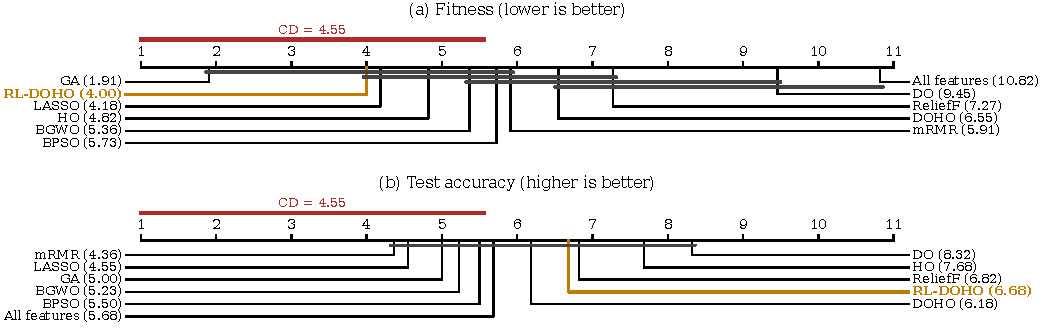
\includegraphics[width=0.92\textwidth]{Fig9}
\caption{Critical-difference diagrams over the eleven datasets (methods ranked by their mean on each dataset; Nemenyi test, $\alpha=0.05$, CD $=4.55$). Thick bars join methods whose average ranks differ by less than the critical difference. Labels are split between the two sides for readability: a method's rank is given by where its line meets the axis (further left is better), not by its label's side or vertical position.}
\label{fig:cd}
\end{figure}

\subsection{Consistency within the DO--HO family}
In Table~\ref{tab:family}, the four family members are ranked against one another run by run.
\begin{itemize}
\item The family-only Friedman test is significant on all eleven datasets, mostly because DO trails the others.
\item RL-DOHO had the best average rank (1.77), ahead of HO (1.89), DOHO (2.63) and DO (3.72). It was the best or tied best of the four in 50\% of runs, against 40\% for HO.
\item RL-DOHO was the worst of the four in only 2 of the 110 runs (HO: 5\%, DOHO: 16\%, DO: 85\% of runs, ties included).
\item Averaged over all 110 runs, RL-DOHO's fitness was 0.0082 above the run's best family member, against 0.0114 for HO. Its single largest gap (0.120, on Glioma) was larger than HO's (0.085).
\end{itemize}
RL-DOHO and HO did not differ significantly in a direct comparison (58 against 49), and on the repeated clinical splits HO had the better family rank (Section~\ref{sec:splits}), so the family ranking shows consistency rather than a clear winner.

\begin{table}[t]
\centering
\caption{Average per-run rank on fitness within the DO--HO family (1 = best of four), family-only Friedman $p$-value per dataset, and how often each method was the best or the worst of the four over the 110 runs (ties counted for every tied method).}
\label{tab:family}
\footnotesize
\setlength{\tabcolsep}{3.5pt}
\begin{tabular}{@{}lccccc@{}}
\toprule
Dataset & RL-DOHO & DO & HO & DOHO & Friedman $p$ \\
\midrule
Rheumatic & \textbf{1.60} & 4.00 & 1.85 & 2.55 & $<$0.001 \\
\midrule
Colon & \textbf{1.75} & 3.45 & 1.90 & 2.90 & 0.007 \\
ALL/AML & \textbf{1.70} & 3.60 & 1.75 & 2.95 & 0.001 \\
Lung & 2.10 & 3.80 & \textbf{1.70} & 2.40 & 0.002 \\
Glioma & \textbf{1.50} & 3.25 & 2.30 & 2.95 & 0.011 \\
GSE93272 & 2.20 & 3.20 & \textbf{1.50} & 3.10 & 0.009 \\
\midrule
WDBC & \textbf{1.50} & 3.85 & 2.30 & 2.35 & $<$0.001 \\
Hepatitis & \textbf{1.80} & 3.95 & 2.05 & 2.20 & $<$0.001 \\
Dermatology & 1.90 & 3.85 & \textbf{1.70} & 2.55 & $<$0.001 \\
SPECTF & \textbf{1.50} & 3.95 & 2.00 & 2.55 & $<$0.001 \\
Backache & 1.90 & 4.00 & \textbf{1.70} & 2.40 & $<$0.001 \\
\midrule
Mean (110 runs) & \textbf{1.77} & 3.72 & 1.89 & 2.63 & -- \\
Best or tied (\%) & \textbf{50} & 3 & 40 & 15 & -- \\
Worst or tied (\%) & \textbf{2} & 85 & 5 & 16 & -- \\
\bottomrule
\end{tabular}
\end{table}

\subsection{Hypotheses H1--H12}
Table~\ref{tab:hyp} reports the hypotheses fixed in advance.
\begin{itemize}
\item \textbf{H1}: supported, and again on the tabular datasets (49 against 1).
\item \textbf{H2}: no significant difference, and none on the tabular data (30 against 20, $p=0.20$).
\item \textbf{H3}: not supported. At $3\times$ budget the bandit won 27 runs against random selection and lost 29; on the tabular data it was 28 to 20 ($p=0.31$).
\item \textbf{H4}: supported.
\item \textbf{H5}: no significant difference between Q-learning and random selection (46 against 56).
\item \textbf{H6}: supported for HO, not for the GA (Section~\ref{sec:addon}).
\item \textbf{H7}: rejected, since the choice of $\kappa$ did change fitness (Section~\ref{sec:kappa}).
\item \textbf{H8}: significant only against DO and against using all features (Section~\ref{sec:splits}).
\item \textbf{H9}: all tested tabular results reproduced with the SVM, PERTURB's advantage among them (Section~\ref{sec:svm}).
\item \textbf{H10a} was not supported: the warm-started bandit was level with random selection (Section~\ref{sec:discussion}).
\item \textbf{H11a/b} were not supported: a reward aimed at the best subset did not make the bandit beat random selection.
\item \textbf{H12a--d} were all supported: RL-DOHO stayed ahead of DO under every change to DO's step size and encoding (Section~\ref{sec:discussion}).
\end{itemize}

\begin{table}[t]
\centering
\caption{Hypotheses fixed in advance: W/T/L for the first-named method and two-sided sign-test $p$ (H6: Holm-corrected over the two comparisons; H7: Friedman test over the four values of $\kappa$; H8: summary of twelve Holm-corrected comparisons; H9: tabular data with an SVM; H10a--H12: the ten KNN datasets; H11 and H12: Holm-corrected within each).}
\label{tab:hyp}
\footnotesize
\setlength{\tabcolsep}{1.7pt}
\begin{tabular}{@{}llccl@{}}
\toprule
& Comparison (fitness) & Runs & W/T/L & $p$ \\
\midrule
H1 & RL-DOHO vs.\ published DO & 60 & 54/3/3 & $<$0.001 \\
H2 & RL-DOHO vs.\ published HO & 60 & 28/3/29 & 1.000 \\
H3 & UCB (gain) vs.\ random, 3$\times$ budget & 60 & 27/4/29 & 0.894 \\
H4 & Sparse vs.\ dense start (gene data) & 50 & 46/0/4 & $<$0.001 \\
\midrule
H5 & Q-learning vs.\ random, 3$\times$ budget & 110 & 46/8/56 & 0.373 \\
H6 & GA+SI vs.\ GA & 110 & 45/16/49 & 0.757 \\
   & HO+SI vs.\ HO & 110 & 71/10/29 & $<$0.001 \\
H7 & $\kappa\in\{1,2,3,4\}$ (Friedman) & 110 & -- & $<$0.001 \\
H8 & RL-DOHO vs.\ each, repeated splits & 15 & Supp.\ Tab.~S3 & -- \\
\midrule
H9a & RL-DOHO vs.\ DO (SVM) & 50 & 50/0/0 & $<$0.001 \\
H9b & RL-DOHO vs.\ HO (SVM) & 50 & 32/0/18 & 0.065 \\
H9c & GA vs.\ RL-DOHO (SVM) & 50 & 43/2/5 & $<$0.001 \\
H9d & HO+SI vs.\ HO (SVM) & 50 & 37/5/8 & $<$0.001 \\
 & GA+SI vs.\ GA (SVM) & 50 & 16/17/17 & 1.000 \\
H9e & RL-DOHO vs.\ PERTURB alone (SVM) & 50 & 8/1/41 & $<$0.001 \\
\midrule
H10a & Warm UCB1 vs.\ random, 3$\times$ & 100 & 46/1/53 & 0.547 \\
H11a & Best-gain UCB1 vs.\ random, 3$\times$ & 100 & 50/2/48 & 0.920 \\
H11b & Same, $c=0.2$ & 100 & 55/3/42 & 0.446 \\
\midrule
H12a & RL-DOHO vs.\ DO, step $\times$10 & 100 & 75/0/25 & $<$0.001 \\
H12b & RL-DOHO vs.\ DO, step $\times$100 & 100 & 61/0/39 & 0.035 \\
H12c & RL-DOHO vs.\ DO, sigmoid & 100 & 85/0/15 & $<$0.001 \\
H12d & Both with step $\times$100 & 100 & 73/7/20 & $<$0.001 \\
\bottomrule
\end{tabular}
\end{table}

\subsection{Ablation and controllers}\label{sec:ablation}
Table~\ref{tab:ablation} and Fig.~\ref{fig:abl} vary one component at a time. In the figure, the published DO (no intervention) ranks last in every group of runs, the three controllers lie close together on the gene and tabular data, and PERTURB alone ranks first on the clinical and tabular data but not on the gene data.
\begin{itemize}
\item \textbf{The interventions:} without them, what remains is essentially the published DO run inside the RL-DOHO loop. This variant was worse in 103 of 110 runs ($p<0.001$) and on all three data types.
\item \textbf{The sparse start:} the dense start was worse in 46 of the 50 gene runs ($p<0.001$). Mean fitness rose from 0.0786 to 0.1269, and the selected subsets grew from about 157 genes to about 870.
\item \textbf{The controller:} with random arm choice, results were level with the bandit on every data type (54 against 51 overall). The random version also beat the fixed DO-then-HO hybrid by about the same margin as the bandit (81--25, compared with 81--28). The Q-learning controller was behind the bandit in 62 runs and ahead in 45 ($p=0.12$); its deficit was largest on the clinical data (8 against 1, $p=0.039$) and absent on the tabular data (23 against 27). It was also level with random selection (44 against 62, $p=0.098$). The old reward gave the same results in 7 of 10 clinical runs and was level on gene data.
\item \textbf{PERTURB alone} was ahead of the full arm set on the clinical (6 against 2) and tabular data (39 against 8, $p<0.001$), and behind it on gene data (19 against 30, $p=0.15$). Over all 110 runs it was ahead in 64 and behind in 40 ($p=0.024$, unadjusted). The advantage is specific to the low-dimensional data, and it replicated with an SVM (Section~\ref{sec:svm}).
\item \textbf{The parsimony tie-break} did not change the outcome of a single clinical run.
\item \textbf{With three times the budget} the three controllers finished level on all data types (Table~\ref{tab:ablation}, bottom). On the clinical data all three reached a mean fitness of about 0.1824 with about 10.4 features, close to the best subset found by any run (0.1820, 10 features).
\end{itemize}

\begin{table}[t]
\centering
\caption{Ablation and controllers. Top: at the standard budget, mean fitness and W/T/L of the full method (UCB1, gain reward) against each variant. Bottom: the controllers at three times the budget. Sign-test $p$ unadjusted. The old reward, the tie-break and the dense start were run in the earlier part of the study only (the dense start applies to gene data only).}
\label{tab:ablation}
\footnotesize
\setlength{\tabcolsep}{3.4pt}
\begin{tabular}{@{}lccccccc@{}}
\toprule
& \multicolumn{2}{c}{Clinical (10 runs)} & \multicolumn{2}{c}{Gene expression (50)} & \multicolumn{2}{c}{Medical tabular (50)} & All (110) \\
\cmidrule(lr){2-3}\cmidrule(lr){4-5}\cmidrule(lr){6-7}\cmidrule(l){8-8}
Variant & Fitness & W/T/L ($p$) & Fitness & W/T/L ($p$) & Fitness & W/T/L ($p$) & W/T/L ($p$) \\
\midrule
RL-DOHO (UCB1, gain reward) & 0.1832 & -- & 0.0786 & -- & 0.1494 & -- & -- \\
Q-learning controller & 0.1846 & 8/1/1 (0.039) & 0.0853 & 31/2/17 (0.059) & 0.1507 & 23/0/27 (0.672) & 62/3/45 (0.122) \\
Random arm & 0.1846 & 6/2/2 (0.289) & 0.0815 & 25/2/23 (0.885) & 0.1487 & 23/1/26 (0.775) & 54/5/51 (0.845) \\
PERTURB only & 0.1825 & 2/2/6 (0.289) & 0.0860 & 30/1/19 (0.152) & 0.1359 & 8/3/39 ($<$0.001) & 40/6/64 (0.024) \\
UCB1, old reward & 0.1836 & 2/7/1 (1.000) & 0.0828 & 23/7/20 (0.761) & -- & -- & -- \\
No tie-break & 0.1832 & 0/10/0 (1.000) & -- & -- & -- & -- & -- \\
Dense start & -- & -- & 0.1269 & 46/0/4 ($<$0.001) & -- & -- & -- \\
No intervention (DO) & 0.2280 & 10/0/0 (0.002) & 0.1113 & 44/3/3 ($<$0.001) & 0.1946 & 49/0/1 ($<$0.001) & 103/3/4 ($<$0.001) \\
\midrule
\multicolumn{8}{@{}l@{}}{\emph{Three times the budget (756 and 3,060 evaluations): UCB1 with the gain reward against each alternative}} \\
\midrule
UCB1, gain reward & 0.1824 & -- & 0.0676 & -- & 0.1372 & -- & -- \\
Q-learning & 0.1824 & 1/4/5 (0.219) & 0.0703 & 29/1/20 (0.253) & 0.1371 & 25/1/24 (1.000) & 55/6/49 (0.624) \\
Random arm & 0.1824 & 4/3/3 (1.000) & 0.0645 & 23/1/26 (0.775) & 0.1379 & 28/2/20 (0.312) & 55/6/49 (0.624) \\
UCB1, old reward & 0.1825 & 3/3/4 (1.000) & 0.0686 & 21/3/26 (0.560) & -- & -- & -- \\
\bottomrule
\end{tabular}
\end{table}



\begin{figure}[t]
\centering
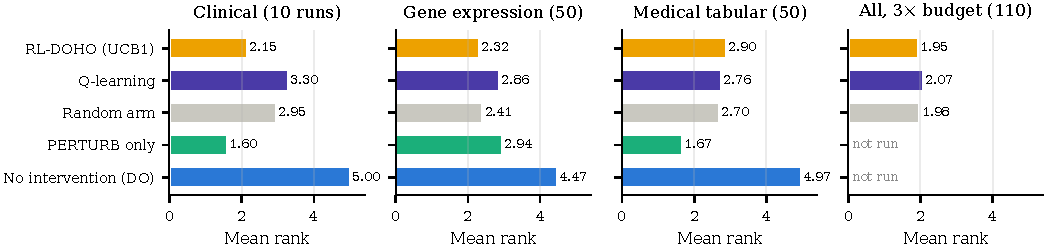
\includegraphics[width=\textwidth]{Fig10}
\caption{Mean per-run fitness rank of the controller variants within each group of runs (lower is better). ``No intervention'' is the published DO; it was not run at three times the budget. Removing the interventions is the only change that is clearly worse everywhere.}
\label{fig:abl}
\end{figure}
\subsection{What the controller did}
Table~\ref{tab:arms} and Fig.~\ref{fig:trace} show how the controller was used in the main runs. In the figure's rheumatic run, DO never leaves its initial best, while RL-DOHO makes its large improvement after about 90 evaluations; on Colon both improve, but RL-DOHO ends lower.
\begin{itemize}
\item \textbf{Clinical runs:} a run contained only 9.4 bandit decisions on average, and four of these were the obligatory first pull of each arm. Its reward-driven choices favoured PERTURB (35\%) and HO (31\%), the two arms that ever lowered the best fitness.
\item \textbf{Gene runs:} there were 27.3 decisions per run, spread almost evenly over the arms. DO exploration steps produced 42\% of the total fitness reduction, PERTURB 26\% and the HO arm 21\%.
\end{itemize}
Different arms carried the search on different problems, yet a random choice among them performed as well as the learned one.

\begin{table}[t]
\centering
\caption{Controller behaviour in the main RL-DOHO runs (10 clinical runs; 50 gene-expression runs over five datasets).}
\label{tab:arms}
\footnotesize
\setlength{\tabcolsep}{5pt}
\begin{tabular}{@{}lcc@{}}
\toprule
& Clinical & Gene expression \\
\midrule
Controller decisions per run & 9.4 & 27.3 \\
\quad of which initial (one per arm) & 4.0 & 4.0 \\
\midrule \multicolumn{3}{l}{\emph{Share of UCB-driven choices (\%)}} \\
\quad PERTURB & 35 & 26 \\
\quad RESTART & 17 & 21 \\
\quad DO & 17 & 28 \\
\quad HO & 31 & 25 \\
\midrule \multicolumn{3}{l}{\emph{Pulls that lowered the best fitness (\%)}} \\
\quad PERTURB & 45 & 16 \\
\quad RESTART & 0 & 2 \\
\quad DO & 0 & 8 \\
\quad HO & 48 & 34 \\
\midrule \multicolumn{3}{l}{\emph{Share of total fitness reduction (\%)}} \\
\quad DO exploration steps & 0.0 & 41.9 \\
\quad PERTURB & 19.5 & 25.6 \\
\quad RESTART & 0.0 & 2.9 \\
\quad DO arm & 0.0 & 8.5 \\
\quad HO arm & 80.5 & 21.1 \\
\bottomrule
\end{tabular}
\end{table}

\begin{figure}[t]
\centering
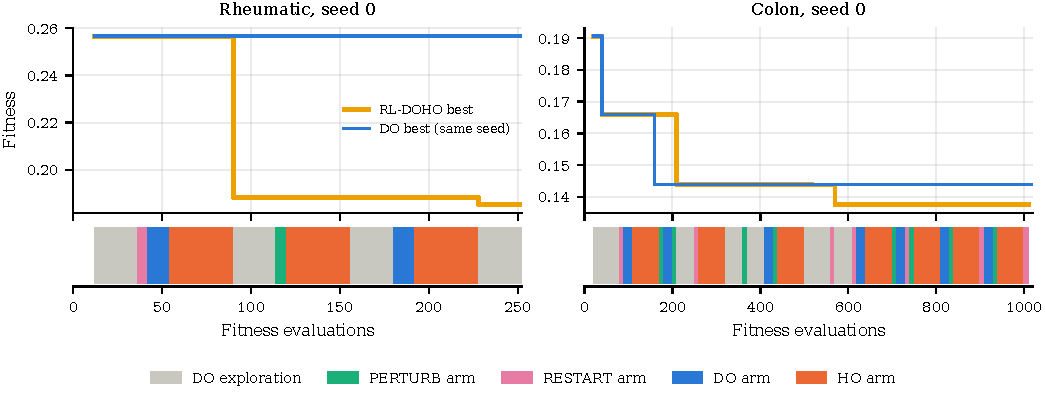
\includegraphics[width=\textwidth]{Fig11}
\caption{Best fitness of RL-DOHO and DO for seed 0 on the rheumatic data and on Colon, against evaluations used, with RL-DOHO's action at each step (bottom). On the rheumatic data DO never improves on its initial best with this seed.}
\label{fig:trace}
\end{figure}

The extension runs show the same picture. The Q-learning controller made 10, 35 and 33 decisions per run on the clinical, gene and tabular data and spread them over all four arms (averaged over runs: DO 33--35\%, PERTURB 27--33\%, RESTART 16--20\%, HO 17--19\%).

\subsection{The intervention layer on GA and HO (H6)}\label{sec:addon}
Table~\ref{tab:addon} and Fig.~\ref{fig:addonk}(a) compare the GA and HO with and without the intervention layer. In panel (a), the changes for HO are mostly below zero (an improvement), while those for the GA scatter around zero.
\begin{itemize}
\item \textbf{HO+SI against HO:} lower fitness in 71 runs and higher in 29 (Holm $p<0.001$). The gain came mostly from the tabular data (40 against 8), with a weaker trend on gene data (30 against 16, $p=0.054$) and none on the clinical data (1 against 5). HO+SI had the lower mean fitness on 8 of the 11 datasets, by up to 16\% (Colon, Glioma, Dermatology).
\item \textbf{GA+SI against the GA:} no difference (45 against 49), on every data type.
\item \textbf{Test accuracy} did not change in either case (HO+SI 39 against 35, GA+SI 34 against 32).
\item \textbf{Against RL-DOHO}, HO+SI was ahead in 61 runs and behind in 47 ($p=0.21$), and GA+SI was ahead in 85 and behind in 25 ($p<0.001$).
\end{itemize}
HO+SI stalled less often than GA+SI and made fewer decisions (4, 12 and 13 per run on the clinical, gene and tabular data, against 15, 47 and 48). Of the fitness reduction achieved during HO+SI's interventions, 69\% came from PERTURB, 27\% from the HO arm and 4\% from RESTART. For GA+SI the GA arm produced 57\% and PERTURB 42\%.

\begin{table}[t]
\centering
\caption{The intervention layer on the GA and HO. Top: mean fitness per data type and mean number of selected features over all 110 runs. Bottom: W/T/L for the first-named method on fitness per data type and over all runs, with sign-test $p$ (Holm-corrected over the two H6 comparisons in the first two rows), and on test accuracy.}
\label{tab:addon}
\footnotesize
\setlength{\tabcolsep}{4pt}
\begin{tabular}{@{}lcccc@{}}
\toprule
Method & Clinical & Gene expression & Medical tabular & Features (all) \\
\midrule
RL-DOHO & 0.1832 & 0.0786 & 0.1494 & 78.7 \\
GA & 0.1821 & 0.0616 & 0.1309 & 62.4 \\
GA+SI & 0.1822 & 0.0627 & 0.1321 & 57.9 \\
HO & 0.1838 & 0.0816 & 0.1534 & 52.7 \\
HO+SI & 0.1839 & 0.0738 & 0.1427 & 54.1 \\
\bottomrule
\end{tabular}

\vspace{2mm}
\begin{tabular}{@{}lccccccc@{}}
\toprule
& \multicolumn{5}{c}{Fitness} & \multicolumn{2}{c}{Test accuracy} \\
\cmidrule(lr){2-6}\cmidrule(l){7-8}
Comparison & Clinical (10) & Gene (50) & Tabular (50) & All (110) & $p$ & All (110) & $p$ \\
\midrule
GA+SI vs.\ GA & 2/5/3 & 25/0/25 & 18/11/21 & 45/16/49 & 0.757 & 34/44/32 & 0.902 \\
HO+SI vs.\ HO & 1/4/5 & 30/4/16 & 40/2/8 & 71/10/29 & \textbf{$<$0.001} & 39/36/35 & 0.728 \\
\midrule
RL-DOHO vs.\ GA+SI & 2/0/8 & 16/0/34 & 7/0/43 & 25/0/85 & \textbf{$<$0.001} & 42/13/55 & 0.223 \\
RL-DOHO vs.\ HO+SI & 6/1/3 & 22/1/27 & 19/0/31 & 47/2/61 & 0.211 & 51/10/49 & 0.920 \\
\bottomrule
\end{tabular}
\end{table}

\begin{figure}[t]
\centering
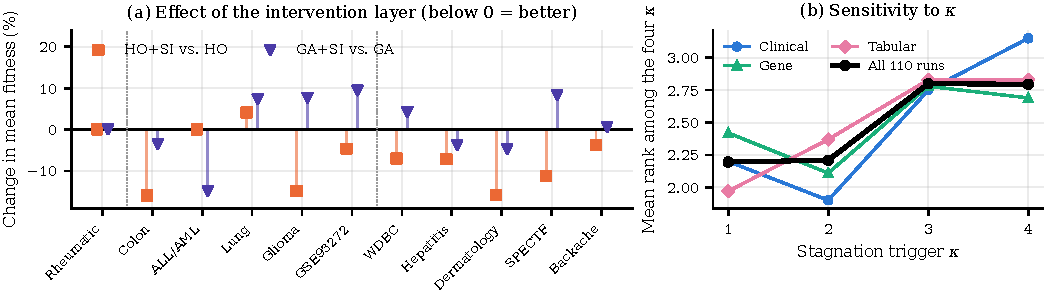
\includegraphics[width=\textwidth]{Fig12}
\caption{(a) Change in mean fitness when the intervention layer is added to HO and to the GA, per dataset (negative is better); dotted lines separate the clinical, gene-expression and tabular datasets. (b) Mean per-run rank of RL-DOHO's fitness among the four values of the stagnation trigger $\kappa$, by data type and over all 110 runs.}
\label{fig:addonk}
\end{figure}

\subsection{Sensitivity to the stagnation trigger (H7)}\label{sec:kappa}
In Table~\ref{tab:kappa} and Fig.~\ref{fig:addonk}(b), $\kappa$ (how many iterations without improvement are tolerated before intervening) is set to 1, 2, 3 and 4.
\begin{itemize}
\item The Friedman test over $\kappa\in\{1,2,3,4\}$ is significant ($\chi^2=23.84$, $p<0.001$), so H7 is rejected.
\item There was no real difference between $\kappa=1$ and the default $\kappa=2$ (mean ranks 2.20 and 2.21; 54 against 50 runs). Waiting longer was worse: $\kappa=3$ lost to $\kappa=2$ in 71 runs and won in 38 ($p=0.002$), and $\kappa=4$ lost in 70 and won in 35 ($p<0.001$).
\item By mean rank, $\kappa=3$ and $\kappa=4$ were worse than $\kappa=2$ on every data type, although the per-type Friedman tests were significant only on gene ($p=0.040$) and tabular data ($p=0.001$). On the tabular data $\kappa=1$ was also better than $\kappa=2$ (31 against 17 runs, $p=0.059$; mean fitness 0.1422 against 0.1494).
\item Test accuracy did not differ between any value of $\kappa$ and the default.
\end{itemize}
The default was fixed before these runs, so the sweep confirms it rather than tuning it.

\begin{table}[t]
\centering
\caption{Sensitivity to the stagnation trigger $\kappa$: mean fitness per data type, mean per-run rank among the four values over 110 runs (Friedman $p<0.001$), and W/T/L against the default $\kappa=2$ with sign-test $p$.}
\label{tab:kappa}
\footnotesize
\setlength{\tabcolsep}{2.6pt}
\begin{tabular}{@{}lcccccc@{}}
\toprule
& \multicolumn{3}{c}{Mean fitness} & & \multicolumn{2}{c}{vs.\ $\kappa=2$} \\
\cmidrule(lr){2-4}\cmidrule(l){6-7}
$\kappa$ & Clinical & Gene & Tabular & Rank & W/T/L & $p$ \\
\midrule
$\kappa=1$ & 0.1836 & 0.0793 & 0.1422 & \textbf{2.20} & 54/6/50 & 0.769 \\
$\kappa=2$ (default) & 0.1832 & 0.0786 & 0.1494 & 2.21 & -- & -- \\
$\kappa=3$ & 0.1855 & 0.0910 & 0.1490 & 2.80 & 38/1/71 & \textbf{0.002} \\
$\kappa=4$ & 0.1857 & 0.0882 & 0.1525 & 2.80 & 35/5/70 & \textbf{$<$0.001} \\
\bottomrule
\end{tabular}
\end{table}

\subsection{Repeated clinical splits (H8)}\label{sec:splits}
Table~S3 of Online Resource~1 gives the full results of repeating the clinical comparison on two further train/test splits.
\begin{itemize}
\item \textbf{RL-DOHO did about as well on split 1 as on the original split, and worse on split 2.} Its average per-run fitness rank among the 13 methods was 5.2 on the original split, 5.3 on split 1 and 9.2 on split 2. On split 2 the best subset found by any run (fitness 0.1785) was found easily: HO and LASSO reached it in all five runs, HO+SI in four and the GA in three, and RL-DOHO in none.
\item \textbf{H8:} over the 15 paired runs, RL-DOHO's fitness differed significantly only from DO (15 against 0) and the full feature set (14 against 1). The GA was ahead in 12 runs and behind in 3 (unadjusted $p=0.035$, Holm $p=0.35$); all other comparisons were closer.
\item \textbf{Test accuracy} differed significantly only from DO. Apart from DO and BGWO, the methods' mean test accuracy lay within 0.4 percentage points of each other on each new split, and RL-DOHO's per-run test-accuracy rank was 5.67, fourth of 13.
\item \textbf{Within the DO--HO family}, HO had the better average rank on these splits (1.53 against 2.03 for RL-DOHO).
\end{itemize}



\subsection{Cost}
Although the budget of fitness evaluations was the same for all methods, a subset seen before is answered from the cache. The number of distinct subsets is therefore the better measure of cost. On the new clinical splits RL-DOHO evaluated 83 per run, against 131 for HO and 132 for the GA (about 5, 8 and 8 minutes at 3.6~s per evaluation). On the tabular data the figures were 381, 596 and 633. A low count is not a quality signal in itself: DO evaluated the fewest distinct subsets and was also the weakest method. Overhead from the search algorithms themselves stayed under 1.5~ms per evaluation in all cases, including $D=7{,}129$. Table~S2 of Online Resource~1 gives the full figures.

\subsection{A second classifier (H9)}\label{sec:svm}
For Table~\ref{tab:svm}, the tabular benchmark was rerun with an RBF-kernel SVM as the wrapped classifier.
\begin{itemize}
\item \textbf{Method ranking.} The mean per-run fitness ranks of the 11 methods under the two classifiers had a Spearman correlation of 0.99; only mRMR and ReliefF swapped places. The GA ranked first (1.58), followed by binary PSO (3.19), binary GWO (3.53), RL-DOHO (3.81) and HO (4.40).
\item \textbf{H9a--H9d replicated.} RL-DOHO beat DO in all 50 runs, was ahead of HO in 32 and behind in 18 ($p=0.065$), and trailed the GA (5 against 43). The intervention layer again improved HO (37 against 8, $p<0.001$) and left the GA unchanged (16 against 17, with 17 ties).
\item \textbf{H9e:} PERTURB alone again reached lower fitness than the full arm set, in 41 runs against 8 ($p<0.001$), on four of the five datasets by at least 8 runs to 2. It did so on WDBC, Dermatology and SPECTF too, so the advantage does not depend on the two weakest datasets.
\item \textbf{Within the DO--HO family}, RL-DOHO had the best average rank (1.54, against 1.79 for HO).
\item \textbf{Test scores:} the SVM's mean test balanced accuracy was similar to 5-NN's (51.8--96.3\% against 53.6--95.5\% across the datasets), and no pooled test-accuracy comparison with RL-DOHO was significant after correction.
\end{itemize}

\begin{table}[t]
\centering
\caption{Medical tabular datasets with an SVM and with 5-NN as the classifier (50 paired runs each, same splits and seeds): W/T/L for the first-named method on fitness and unadjusted two-sided sign-test $p$. Bold: $p<0.05$.}
\label{tab:svm}
\footnotesize
\setlength{\tabcolsep}{2.6pt}
\begin{tabular}{@{}lcccc@{}}
\toprule
& \multicolumn{2}{c}{SVM} & \multicolumn{2}{c}{5-NN} \\
\cmidrule(lr){2-3}\cmidrule(l){4-5}
Comparison & W/T/L & $p$ & W/T/L & $p$ \\
\midrule
RL-DOHO vs.\ DO & 50/0/0 & \textbf{$<$0.001} & 49/0/1 & \textbf{$<$0.001} \\
RL-DOHO vs.\ HO & 32/0/18 & 0.065 & 30/0/20 & 0.203 \\
RL-DOHO vs.\ DOHO & 40/2/8 & \textbf{$<$0.001} & 35/0/15 & \textbf{0.007} \\
GA vs.\ RL-DOHO & 43/2/5 & \textbf{$<$0.001} & 45/1/4 & \textbf{$<$0.001} \\
RL-DOHO vs.\ BPSO & 20/3/27 & 0.382 & 20/0/30 & 0.203 \\
RL-DOHO vs.\ BGWO & 21/2/27 & 0.471 & 20/0/30 & 0.203 \\
RL-DOHO vs.\ LASSO & 41/0/9 & \textbf{$<$0.001} & 38/0/12 & \textbf{$<$0.001} \\
\midrule
HO+SI vs.\ HO & 37/5/8 & \textbf{$<$0.001} & 40/2/8 & \textbf{$<$0.001} \\
GA+SI vs.\ GA & 16/17/17 & 1.000 & 18/11/21 & 0.749 \\
PERTURB only vs.\ RL-DOHO & 41/1/8 & \textbf{$<$0.001} & 39/3/8 & \textbf{$<$0.001} \\
\bottomrule
\end{tabular}
\end{table}


\subsection{Sensitivity to the operator implementation}
The first version of this study differed in three ways: simplified DO and HO update rules, a dense start on every dataset, and a budget counted in iterations. On the six datasets of the main study the conclusions about the DO--HO family and the GA were the same under both versions: RL-DOHO was clearly better than DO, level with HO and behind the GA. Only the comparison with binary PSO and GWO reversed, most likely because of the sparse start. Section~S1 of Online Resource~1 gives the details.



\section{Discussion}\label{sec:discussion}

\subsection{RL-DOHO supplies the moves that DO lacks}
With the binary encoding used here, a feature changes only when its coordinate crosses zero. In every iteration the landing stage of the published DO drags the whole population back to within a small Lévy step of the elite. With only 14 features, that nearly always recreates the elite's subset, and it is why DO got past its initial best in just one clinical run. On gene data, with thousands of coordinates, the heavy tails of the Lévy steps do flip some features, and DO improved in 48 of 50 runs, but slowly. RL-DOHO's interventions supply exactly what DO lacks under this encoding: new subsets near the best one (PERTURB), new subsets elsewhere (RESTART), and HO's greedy, randomized moves. The ablation fits this explanation, since taking the interventions out made 103 of 110 runs worse. Because this explanation makes DO weak partly by construction, we tested it (H12). Larger landing steps did help DO: with a 10$\times$ or 100$\times$ step it beat the published DO in 83 and 84 of 100 runs and evaluated far more distinct subsets (193--382 per tabular run with the 100$\times$ step, against 22--26). The standard sigmoid transfer function helped less (60 against 40, $p=0.057$) and, on gene data, selected hundreds to thousands of genes. RL-DOHO nevertheless stayed ahead of every variant: 75 against 25 runs for the 10$\times$ step, 85 against 15 for the sigmoid, and 61 against 39 for the 100$\times$ step (Holm $p=0.035$). The last was level on the tabular data (24 against 26) and decided by the gene data (37 against 13). When both used the 100$\times$ step, the layer still improved DO in 73 runs against 20 ($p<0.001$), on tabular and gene data alike. The published step size is therefore part of why DO is weak, but it is not the reason RL-DOHO beats it, and RL-DOHO itself was unchanged by the larger step (50 against 49). No test-accuracy difference in these comparisons was significant. Section~S6 of Online Resource~1 gives the details.

\subsection{The interventions help optimizers that lack local moves}
The add-on experiment tests the interventions without DO. Wrapped around HO they lowered fitness in 71 of the 100 decided runs, while around the GA they made no difference. It is not that the GA never stalls. GA+SI actually intervened more often, 47--48 times per gene or tabular run compared with 12--13 for HO+SI. The relevant difference is in the base optimizers' own moves after a stall. A GA generation recombines and mutates good subsets directly in the binary space, and within GA+SI's interventions the GA arm itself produced 57\% of the fitness reduction, so the extra moves largely duplicated what the GA already does. HO behaves differently. An HO iteration (about $3N$ evaluations) moves continuous positions relative to a dominant agent, and none of its phases samples the immediate neighbourhood of the best subset. That neighbourhood is what PERTURB searches, at a cost of $N/2$. Our reading is that the interventions are useful when they give the base optimizer a type of move it does not have, and not as a general improvement to wrapper search.

Among the interventions, PERTURB, a bit-flip local search around the best subset, is the most useful on low-dimensional data. It produced 69\% of the fitness reduction during HO+SI's interventions (42\% in GA+SI), and PERTURB alone beat the full arm set on the tabular data with both classifiers (39 against 8 runs with 5-NN, 41 against 8 with an SVM) and was ahead on the clinical data too, although not significantly (6 against 2). On gene data, where a few bit flips change little among thousands of features, the full arm set was ahead (30 against 19, not significant), and in RL-DOHO's main gene runs DO exploration steps produced more of the improvement than PERTURB. The $\kappa$ results are consistent with this: $\kappa=1$ or 2 gave lower fitness than $\kappa=3$ or 4. A practical reading is that a stalled population-based search should be followed quickly by a short local search around its best subset; on our tabular datasets (19--44 features) that local search alone was the better choice overall, although not on every dataset (for example Hepatitis with the SVM, 5 against 4), and on gene data it was not. The fitness advantage of PERTURB alone did not show up in test accuracy (19 against 26 runs with 5-NN, 21 against 22 with an SVM), in line with the other comparisons.

\subsection{Learned move selection does not outperform random choice}
The controller result now holds for three controllers (UCB1, a stateful Q-learner and random selection), three reward designs, three data types and two budgets, so it is unlikely to be an artefact of a single setting. Two explanations seemed plausible. One is that the arms complement each other instead of one being clearly best, in which case picking at random costs little. The other is that there are simply too few decisions to learn from. With the standard budget the bandit decided only 9 times in a clinical run, 4 of them forced initial pulls, and about 30 times in a gene or tabular run, while the Q-learner had 10 to 35 decisions to fill six states. So few decisions leave a learned preference little time to pay off. The Q-learner was slightly behind the bandit, as one would expect when roughly one decision in six is spent on random exploration. We therefore describe RL-DOHO's controller as an adaptive selector that costs almost nothing and removes the need to fix the move in advance. It did not beat random selection on our data; what makes the method work is the interventions and the initialization.

We tested the second explanation directly (H10a). At $3\times$ budget (about 80--115 decisions per run), UCB1 initialised from two earlier runs on the same training data was no better than random selection (46 against 53 runs, $p=0.55$) and slightly worse than UCB1 started from scratch (39 against 61, unadjusted $p=0.035$, Holm $p=0.070$). The warm-up runs also added about 70\% to the number of distinct evaluations. The bandit started from scratch was once again level with random selection (51 against 46).

A diagnostic recorded in the same runs shows why more decisions did not help, and it also rules out the first explanation in its simple form. First, the arms were not interchangeable: under random selection their rewards differed significantly on every dataset (Kruskal--Wallis, \citealp{kruskal1952}; $p<0.001$). Second, the bandit ordered its choices exactly by mean reward, with a Spearman correlation \citep{spearman1904} of 1.0 between choice frequency and mean reward on each of the ten datasets. The bandit therefore learned what it was rewarded for. The reward, however, did not rank the moves by what matters. DO iterations earned the highest mean reward (0.10--0.13), largely through the population term of the reward, yet improved the best subset in at most 11\% of uses, whereas PERTURB and HO did so in up to 28\% and 22\%. The reward differences were also small relative to UCB1's exploration term, which kept the choice shares close to uniform (DO 32\%, PERTURB 25\%, HO 22\%, RESTART 20\%). With a reward that favours the wrong arm and differences this small, a learned choice can hardly do better than chance. We then tested both fixes together (H11, fixed after the H10a diagnostics): a reward that credits only improvement of the best subset, with the default exploration constant and with $c=0.2$. Under the new reward, the bandit's choices moved towards the arms that actually improved the best subset. Its choice frequencies now tracked how often each move improved the best subset (mean Spearman correlation 0.73, and 0.84 with $c=0.2$, against 0.08 with the original reward), and PERTURB became its most used move (28\%, and 36\% with $c=0.2$). Yet neither variant beat random selection (50 against 48 runs, $p=0.92$; 55 against 42, Holm $p=0.45$), and the share of decisions that improved the best subset hardly changed (7.1--7.6\%, against 7.4\% for random choice). The new reward was ahead of the original one in 57 runs and behind in 37 (unadjusted $p=0.050$, Holm $p=0.15$), a trend at most. The reason is the size of the signal. The limiting factor is how rarely any arm succeeds. The best arm improved the best subset in at most 28\% of its uses and most arms far less often, so over about 100 decisions a preference for it changes the expected outcome only marginally. The bandit identifies the better arm; the better arm is just not much better. The other pre-specified extensions, a move pool with removal and swap moves and a contextual bandit (LinUCB; \citealp{li2010linucb}), are implemented (Section~S3 of Online Resource~1) but were not run.

\subsection{RL-DOHO matches HO and trails the GA on fitness}
RL-DOHO and HO reached statistically indistinguishable fitness (58 against 49 over 110 runs), although RL-DOHO had the better family rank and was rarely the worst of the four. On the repeated clinical splits HO had the better family rank. The GA reached lower fitness than RL-DOHO more often on every data type (85 against 22 overall). Its uniform crossover recombines good subsets directly in the binary space, and with a mutation rate of $1/D$ it stays close to sparse subsets once it starts there; neither property depends on a continuous-to-binary mapping. On test accuracy the GA and RL-DOHO did not differ (48 against 48).

One may ask why we do not just use the GA. On fitness alone, the GA is the better choice on these datasets, and we do not claim otherwise. Even so, three of our results bear on that choice. First, the fitness advantage of the GA was not visible on held-out data (no test-accuracy difference survived correction). Second, the GA was more expensive. It evaluated 59--66\% more distinct subsets than RL-DOHO per run (132 against 83 on the clinical splits, 633 against 381 on the tabular data), which is what counts when each evaluation means training a model. Third, the GA does not need the layer, and the add-on experiment shows why. GA+SI is a memetic GA in the usual sense, a GA with a local search triggered when it stalls, and it was no better than the plain GA (45 against 49). The GA's crossover and mutation already supply the local moves the layer adds. The layer pays off on optimizers that lack such moves, such as DO and HO, and that is the paper's main claim. It is not a claim that RL-DOHO is the best feature selector.

\subsection{Filter fitness on gene data is optimistic}
How the filters compared depended on the kind of data. On gene data LASSO reached lower fitness than every wrapper on every dataset, and mRMR did so on ALL/AML and Lung. On the tabular and clinical data, with 14--44 features, the wrappers led and LASSO, mRMR and ReliefF trailed RL-DOHO. Some of that advantage on gene data is flattering to the filters, though. Their subset size was chosen by minimizing the same cross-validated score that is reported as fitness, the selection bias described by \citet{ambroise2002}. Glioma shows the effect most clearly: LASSO had the best fitness and the worst test accuracy. On held-out data the differences shrink: in the pooled tests over all 110 runs no test-accuracy difference survived correction, and LASSO's lead over RL-DOHO on macro-F1 was the only test-score difference that did.

\subsection{The clinical data do not separate the methods}
On the rheumatic data all methods except the published DO reached test accuracy within about 1.1 points of each other on the original split and, apart from BGWO, within 0.4 points on each new split, and the best subsets were found by many methods. The dataset is too easy to separate the better search methods, which is also why the intervention layer made no difference to HO or the GA there. The two variables that RL-DOHO, the GA, BPSO and BGWO mostly dropped, anti-dsDNA and anti-Sm, are the two with the most missing values (39\% and 43\%). Their low value in this dataset may therefore reflect missingness and mode imputation rather than clinical irrelevance. At equal test accuracy, RL-DOHO's lower number of distinct subsets matters in practice when evaluations are expensive, which was the case for the boosted models on this dataset.

\subsection{Limitations}
Several limitations qualify these results. The clinical findings come from a single cohort, now evaluated on three train/test splits with five seeds each, so they describe this cohort rather than rheumatic diagnosis in general, and validation on an external cohort is still needed. The tabular datasets, the add-on experiment, the Q-learning controller, the $\kappa$ sweep and the SVM runs were designed after the main results were known; their hypotheses were fixed before they were run, but the choice of what to test was informed by the earlier findings. The evaluation budgets (252 and 1,020 fitness evaluations) are modest, and only the controllers were examined at a larger budget. Test sets of 15--171 samples on the gene and tabular data make test scores coarse, which is why we give more weight to fitness and to the pooled tests. The tabular benchmark was repeated with an SVM, but the gene-expression and clinical data were each evaluated with a single classifier configuration (5-NN, and XGBoost with gradient boosting on a 4,000-patient subsample), and no classifier was tuned. RL-DOHO's settings other than $\kappa$, including $\varepsilon$ and the UCB constant, and the Q-learning settings were fixed rather than tuned, which keeps the comparison even but leaves their sensitivity open. Our DO and HO follow the published equations, but the original papers leave some details open (such as the random-group size in HO), so other implementations may behave differently. The cost figures come from one shared cloud runtime. We did not reimplement recent binary HO variants such as Q2HO-MFTV \citep{hashjin2025q2ho}, so the comparison with learned strategy selection inside HO rests on our own Q-learning ablation. Two of the tabular datasets (Backache and Hepatitis) are close to chance for 5-NN; Table~\ref{tab:weak} shows which conclusions depend on them. Finally, the filter methods chose their subset size on the same cross-validated score that is reported as fitness, which favours them on that measure, and the pooled sign tests treat runs on the same dataset as independent and combine datasets of different size and difficulty. They are best read together with the per-dataset results and the dataset-level ranks, on which RL-DOHO is separated only from DO and the full feature set.


\section{Conclusion}
We presented a stagnation-triggered intervention layer for wrapper feature selection and its instantiation, RL-DOHO. RL-DOHO runs the published DO while the best subset improves and, after $\kappa=2$ stalled iterations, lets a UCB1 bandit choose among a bit-flip search, a partial restart, a DO iteration and an HO iteration. The evaluation covered eleven datasets with ten seeds each, equal evaluation budgets for all methods, and hypotheses fixed before the corresponding runs. Main findings:
\begin{itemize}
\item \textbf{Against DO:} RL-DOHO won 103 of the 110 paired runs on fitness and lost 4. Its lead held against DO with 10$\times$ and 100$\times$ larger L\'evy steps (75 against 25 and 61 against 39 runs) and with a sigmoid transfer function (85 against 15). Even a DO that already used the larger step was improved by the layer (73 against 20).
\item \textbf{Against the other baselines:} it came out ahead of the fixed DO-then-HO hybrid (81 against 28), of binary PSO (70 against 38) and of the ReliefF (84 against 26) and mRMR (68 against 40) filters, although the mRMR result did not hold without the two weakest tabular datasets (48 against 40, $p=0.46$). It was not significantly different from HO (58 against 49), binary GWO (67 against 43, Holm $p=0.084$) or LASSO (49 against 61). It had the best average rank in the DO--HO family (1.77, against 1.89 for HO) and was the family's worst member in only 2 of 110 runs. The GA reached lower fitness in 85 runs against 22.
\item \textbf{The layer on other optimizers:} it improved HO in 71 runs against 29 ($p<0.001$; 37 against 8 with an SVM) and left the GA unchanged (45 against 49).
\item \textbf{The controller:} UCB1 was level with random choice (54 against 51), and so was Q-learning at $3\times$ budget (46 against 56). The same held for a warm-started UCB1 (46 against 53) and for a UCB1 rewarded only for improving the best subset (50 against 48). Under that reward the choice frequencies followed each move's success rate (Spearman 0.73--0.84, against 0.08 with the original reward), but no move succeeded in more than 28\% of its uses.
\item \textbf{Trigger and moves:} $\kappa=1$ or 2 beat $\kappa=3$ or 4 (Friedman $p<0.001$). On the tabular data the bit-flip search alone beat the full set of moves (39 against 8 runs with 5-NN, 41 against 8 with an SVM), but not on gene data (19 against 30).
\item \textbf{Robustness and cost:} with an SVM instead of 5-NN the method ranking was almost the same (Spearman 0.99). Over three clinical train/test splits, RL-DOHO differed significantly only from DO and the full feature set. On the clinical and tabular data it evaluated 35--40\% fewer distinct subsets than HO or the GA (83 against 131 and 132 per clinical run).
\item \textbf{Held-out data:} after correction, none of the pooled test-accuracy differences remained significant.
\end{itemize}
Future work should test the layer on more clinical cohorts with external validation, test learned controllers on move pools whose members differ more in success rate, and examine binary encodings under which the published DO can move more freely.

\backmatter

\section*{Declarations}

\begin{itemize}
\item \textbf{Funding.} The authors did not receive support from any organization for the submitted work.
\item \textbf{Competing interests.} The authors have no competing interests to declare that are relevant to the content of this article.
\item \textbf{Ethics approval and consent to participate.} Not applicable. The study uses only publicly available, de-identified datasets.
\item \textbf{Consent for publication.} Not applicable.
\item \textbf{Data availability.} The rheumatic and autoimmune disease dataset is openly available under a CC BY 4.0 licence \citep{mahdi2025data}. The microarray datasets are available from the scikit-feature repository \citep{li2017fs}, GSE93272 from the NCBI Gene Expression Omnibus, and the five tabular datasets from PMLB \citep{olson2017pmlb}. The per-run results behind every table and figure are available at \url{https://github.com/adj-04/rl-doho}.
\item \textbf{Code availability.} The notebooks and analysis scripts used in this study are available at \url{https://github.com/adj-04/rl-doho}.
\item \textbf{Author contributions.} Preetha Evangeline D: conceptualization, supervision, writing -- review and editing. Prasenjit Choudhury: methodology, software, investigation, formal analysis, writing -- original draft. Shreyansh Dabgar: software, investigation, validation, writing -- review and editing. Aditya Jha: software, data curation, investigation, writing -- review and editing. All authors read and approved the final manuscript.
\end{itemize}

\bibliography{refs}

\end{document}
